% This is the Reed College LaTeX thesis template. Most of the work
% for the document class was done by Sam Noble (SN), as well as this
% template. Later comments etc. by Ben Salzberg (BTS). Additional
% restructuring and APA support by Jess Youngberg (JY).
% Your comments and suggestions are more than welcome; please email
% them to cus@reed.edu
%
% See http://web.reed.edu/cis/help/latex.html for help. There are a
% great bunch of help pages there, with notes on
% getting started, bibtex, etc. Go there and read it if you're not
% already familiar with LaTeX.
%
% Any line that starts with a percent symbol is a comment.
% They won't show up in the document, and are useful for notes
% to yourself and explaining commands.
% Commenting also removes a line from the document;
% very handy for troubleshooting problems. -BTS

% As far as I know, this follows the requirements laid out in
% the 2002-2003 Senior Handbook. Ask a librarian to check the
% document before binding. -SN

%%
%% Preamble
%%
% \documentclass{<something>} must begin each LaTeX document
\documentclass[12pt,oneside,a4paper]{reedthesis}
% Packages are extensions to the basic LaTeX functions. Whatever you
% want to typeset, there is probably a package out there for it.
% Chemistry (chemtex), screenplays, you name it.
% Check out CTAN to see: http://www.ctan.org/
%%
\usepackage{graphicx,latexsym}
\usepackage{amsmath}
\usepackage{amssymb,amsthm}
\usepackage{longtable,booktabs,setspace}
\usepackage{chemarr} %% Useful for one reaction arrow, useless if you're not a chem major
\usepackage[hyphens]{url}
% Added by CII
\usepackage{hyperref}
\usepackage{lmodern}
\usepackage{float}
\floatplacement{figure}{H}
% End of CII addition
\usepackage{rotating}

% Next line commented out by CII
%%% \usepackage{natbib}
% Comment out the natbib line above and uncomment the following two lines to use the new
% biblatex-chicago style, for Chicago A. Also make some changes at the end where the
% bibliography is included.
%\usepackage{biblatex-chicago}
%\bibliography{thesis}


% Added by CII (Thanks, Hadley!)
% Use ref for internal links
\renewcommand{\hyperref}[2][???]{\autoref{#1}}
\def\chapterautorefname{Chapter}
\def\sectionautorefname{Section}
\def\subsectionautorefname{Subsection}
% End of CII addition

% Added by CII
\usepackage{caption}
\captionsetup{width=5in}
% End of CII addition

% \usepackage{times} % other fonts are available like times, bookman, charter, palatino

% Syntax highlighting #22

% To pass between YAML and LaTeX the dollar signs are added by CII
\title{Impact of Sample Sizes on the Accuracy of Estimates for a Two-level Logistic Regression Model}
\author{Rasel Biswas}
% The month and year that you submit your FINAL draft TO THE LIBRARY (May or December)
\date{August 2019}
\division{Institute of Statistical Research and Training}
\advisor{Noor Jahan Akter}
\institution{University of Dhaka}
\degree{Bachelor of Science, B.S.(Hons)}
%If you have two advisors for some reason, you can use the following
% Uncommented out by CII
% End of CII addition

%%% Remember to use the correct department!
\department{Applied Statistics}
% if you're writing a thesis in an interdisciplinary major,
% uncomment the line below and change the text as appropriate.
% check the Senior Handbook if unsure.
%\thedivisionof{The Established Interdisciplinary Committee for}
% if you want the approval page to say "Approved for the Committee",
% uncomment the next line
%\approvedforthe{Committee}

% Added by CII
%%% Copied from knitr
%% maxwidth is the original width if it's less than linewidth
%% otherwise use linewidth (to make sure the graphics do not exceed the margin)
\makeatletter
\def\maxwidth{ %
  \ifdim\Gin@nat@width>\linewidth
    \linewidth
  \else
    \Gin@nat@width
  \fi
}
\makeatother

%Added by @MyKo101, code provided by @GerbrichFerdinands

\renewcommand{\contentsname}{Table of Contents}
% End of CII addition

\setlength{\parskip}{0pt}

% Added by CII

\providecommand{\tightlist}{%
  \setlength{\itemsep}{0pt}\setlength{\parskip}{0pt}}

\Acknowledgements{
First of all, I am grateful to the one true God for the good health and wellbeing that were necessary to complete this project. I wish to express my sincere gratitude to my project supervisor Ms.~Noor Jahan Akter. I would also like to thank my friends and classmates for offering me advice, and supporting me through this entire process. Special thanks to my friends and brothers from Fazlul Huq Muslim Hall. Without their help and support, I could not have made it this far. Finally, I must express my very profound gratitude to my parents for providing me with unfailing support throughout my years of study. Thank you.
}

\Dedication{
To my parents.
}

\Declaration{
I, Md. Rasel Biswas hereby formally declare that I have written the submitted Master`s thesis entirely by myself without anyone else's assistance. Where I have drawn on literature or other sources, either in direct quotes, or in paraphrasing such material, I have referenced the original author or authors and the source in which it appeared.
\hfill\break
\hfill\break
\hfill\break
\begin{flushleft}
\rule{0.3\textwidth}{0.4pt}
\end{flushleft}
\begin{flushleft}
  Md. Rasel Biswas\\
  Dhaka, August 2019
\end{flushleft}
}

\Abstract{
In a multilevel framework an important problem is calculating an adequate sample size that generates accurate estimates. Several researches have investigated the behavior of estimates in finite samples, particularly for continuous dependent variables. On the other hand, binary response multilevel models have been investigated less widely. In this research we investigate the sample behavior of estimates in a binary response multilevel model. Particularly, we analyze the influence of different factors on the accuracy of estimates and their profile likelihood confidence intervals for a 2-level logistic regression model, through a Monte Carlo simulation study. We investigate the hypothesis of: (a) different level-1 sample sizes; (b) different level-2 sample sizes; (c) different intra-class correlation coefficients. We investigate the bias of estimates by relative bias and, through a non-coverage indicator, the accuracy of the confidence interval. In all instances we have examined, the point estimates are unbiased (even with very small sample sizes), while the variance components are always underestimated. Despite some exceptions for the variance components, the profile likelihood confidence interval performs very well in all simulated conditions.
}

	\linespread{1.3}
\usepackage{hyperref}
\hypersetup{colorlinks = true, linkcolor = blue, anchorcolor = blue, citecolor = blue, filecolor = blue, urlcolor = blue}
\usepackage{placeins}
% End of CII addition
%%
%% End Preamble
%%
%
\begin{document}

% Everything below added by CII
  \maketitle

\frontmatter % this stuff will be roman-numbered
\pagestyle{empty} % this removes page numbers from the frontmatter
  \begin{abstract}
    In a multilevel framework an important problem is calculating an adequate sample size that generates accurate estimates. Several researches have investigated the behavior of estimates in finite samples, particularly for continuous dependent variables. On the other hand, binary response multilevel models have been investigated less widely. In this research we investigate the sample behavior of estimates in a binary response multilevel model. Particularly, we analyze the influence of different factors on the accuracy of estimates and their profile likelihood confidence intervals for a 2-level logistic regression model, through a Monte Carlo simulation study. We investigate the hypothesis of: (a) different level-1 sample sizes; (b) different level-2 sample sizes; (c) different intra-class correlation coefficients. We investigate the bias of estimates by relative bias and, through a non-coverage indicator, the accuracy of the confidence interval. In all instances we have examined, the point estimates are unbiased (even with very small sample sizes), while the variance components are always underestimated. Despite some exceptions for the variance components, the profile likelihood confidence interval performs very well in all simulated conditions.
  \end{abstract}
  \hypersetup{linkcolor=black}
  \setcounter{tocdepth}{2}
  \tableofcontents

  \listoftables

  \listoffigures
  \begin{acknowledgements}
    First of all, I am grateful to the one true God for the good health and wellbeing that were necessary to complete this project. I wish to express my sincere gratitude to my project supervisor Ms.~Noor Jahan Akter. I would also like to thank my friends and classmates for offering me advice, and supporting me through this entire process. Special thanks to my friends and brothers from Fazlul Huq Muslim Hall. Without their help and support, I could not have made it this far. Finally, I must express my very profound gratitude to my parents for providing me with unfailing support throughout my years of study. Thank you.
  \end{acknowledgements}
  \begin{declaration}
    I, Md. Rasel Biswas hereby formally declare that I have written the submitted Master`s thesis entirely by myself without anyone else's assistance. Where I have drawn on literature or other sources, either in direct quotes, or in paraphrasing such material, I have referenced the original author or authors and the source in which it appeared.
    \hfill\break
    \hfill\break
    \hfill\break
    \begin{flushleft}
    \rule{0.3\textwidth}{0.4pt}
    \end{flushleft}
    \begin{flushleft}
      Md. Rasel Biswas\\
      Dhaka, August 2019
    \end{flushleft}
  \end{declaration}
  \begin{dedication}
    To my parents.
  \end{dedication}
\mainmatter % here the regular arabic numbering starts
\pagestyle{fancyplain} % turns page numbering back on

\hypertarget{intro}{%
\chapter{Introduction}\label{intro}}

\hypertarget{background}{%
\section{Background}\label{background}}

Most of the statistical inference is based on replicated observations of units of analysis of one type (e.g., a sample of individuals, countries, or schools). The analysis of such observations usually is based on the assumption that either the sampled units themselves or the corresponding residuals in some statistical model are independent and identically distributed. However, many kinds of data, including social surveys, have a hierarchical or clustered structure, which includes units of analysis of more than one type. For instance, in educational research, researchers often study how students' academic outcomes are associated with the characteristics of their families, classrooms, and schools. The student test scores are frequently modeled as the result of a combination of individual-level characteristics such as student socioeconomic status (SES) and IQ score, classroom level characteristics, such as the number of students in a classroom, and school-level characteristics, such as the expertise of the teachers or location of the school (Urban, Semi-urban or Rural). In this study, pupils, teachers, classrooms, and schools might all be important units of analysis. Frequently, but by no means always, units of analysis of different types are hierarchically nested (e.g., pupils are nested in classrooms, which, in turn, are nested in schools). Other examples involve organizational research, with employees nested within firms; cross-national comparative research with individuals nested within countries; medical research with patients nested within clinics; and longitudinal research with repeated measures nested within individuals.
Since these analyses include the units of analysis of more than one type, the traditional statistical techniques (i.e., ordinary least squares regression) can not be used in these cases. Multilevel analysis is a general term referring to statistical methods appropriate for the analysis of data sets comprising several types of units of analysis. The levels in the multilevel analysis are another name for the different types of unit of analysis (Goldstein, 2003).

Multilevel analysis, originally developed in the fields of education, sociology, and demography, has received increasing attention in other fields like public health and epidemiology over the past few years. Multilevel analysis has become popular in many fields that have hierarchically organized data in units of analysis at two or more levels. Multilevel analysis can be used either to adjust for the dependency of the observations within clusters by using variables at higher levels, or assessing the impact of higher-level characteristics on the outcome variables after controlling for individual characteristics at a base level (Snijders \& Bosker, 1999).

An important problem that occurs in the practice of the multilevel model is the choice of sample sizes at different levels. Applied practitioners designing a research study are often concerned with the required sample size necessary to estimate unbiased fixed effects and variance components, avoid model convergence issues, and yield accurate confidence intervals around point estimates.
Insufficient sample sizes may lead to biased estimates and/or significance tests with low statistical power (Hox, 2010). Since the 1990s, sample size considerations in multilevel studies have become the topic of a huge amount of contributions.
There are plenty of researches on sample size determination for continuous response multilevel model. However, few studies have been carried out to date that has focused on determining sample sizes for the binary response multilevel model.

\hypertarget{literature}{%
\section{Literature review}\label{literature}}

There is a somewhat wide literature about simulation and studies on this issue for continuous response multilevel models. The robustness issue and the choice of sample size in the multilevel regression model for continuous outcome variable have been studied by several authors (Akter \& Khan, 2018; Clarke \& Wheaton, 2007; Hox, 1998; Kreft, 1996; Maas \& Hox, 2004, 2005; Mok, 1995).
The overall conclusion from these studies is that the estimates of the regression coefficients are nearly unbiased, however, the variance components tend to be biased downward (underestimated) when the number of level 2 units is small (e.g., less than 30) (Maas \& Hox, 2004, 2005). These simulation studies also indicate that a larger number of groups is more important than a larger number of individuals per group (Hox, 2010; Maas \& Hox, 2004).
For two-stage hierarchical linear models, Akter \& Khan (2018) recommend a minimum of 30 groups with 15 units per each group for drawing a valid conclusion about the population.

However, few studies have assessed the accuracy of estimates, sample size or power analysis in multilevel regression for a binary outcome variable. Austin (2005) used Monte Carlo simulation methods to examine the impact of misspecification of the distribution of the random effects on estimation of and inference about both the fixed effects and the random effects in multilevel logistic regression models. He concluded that estimation and inference concerning the fixed effects were insensitive to misspecification of the distribution of the random effects, however, estimation and inferences concerning the random effects were affected by model misspecification. Sastry, Ghosh-Dastidar, Adams, \& Pebley (2006) calculate power and sample size in multilevel logistic regression models for their survey of children, families, and communities in Los Angeles. Based on simulation studies, they decided to sample 65 groups each of size 50.

Moineddin, Matheson, \& Glazier (2007) perform some simulation studies on a random slope logistic model using the AGQ with automatic selection of the number of quadrature points as the estimation procedure. Differently from the continuous case, they suggest a ``50/50'' rule (a minimum of 50 groups with at least 50 units per group) for achieving sufficient accuracy. The estimates of all random components, as well as their standard errors, are underestimated, even with very large sample size. They also investigate how the prevalence of the outcome affects the accuracy of individual-level parameter estimates, finding that group size should be properly adjusted in case of low prevalent outcomes. Furthermore, their results signal some rather low percentages of model convergence in some studies, particularly with low group sizes.

Paccagnella (2011) found that the regression parameter estimates appear unbiased even with small sample size, while the variance components are underestimated. The bias decreases as the number of groups increases. Like continuous response multilevel models, the accuracy of the standard errors of the regression parameter estimates is achieved with a number of groups equal to 50. Unlike continuous response models, the accuracy of the standard errors of variance estimates needs a very large number of groups.
The simulation studies of Moineddin et al. (2007) and Paccagnella (2011) investigated the effect of sample size based on the asymptotic theory, i.e., they assumed that the sample size is sufficiently large to conduct the significance test. Even though the sample size is large enough, testing a variance component using their standard error is woefully inadequate (Bates, 2010).

\hypertarget{motivation-of-the-study}{%
\section{Motivation of the study}\label{motivation-of-the-study}}

A Wald-type confidence interval construction is based on the asymptotic normality of the maximum likelihood estimate. It is well known, however, that properties of estimates in small samples can be very different from the asymptotic properties. A more robust construction of confidence interval is profile likelihood-based confidence interval. Profile likelihood works well in both situations when the sample size is small and variance components are to be estimated (Venzon \& Moolgavkar, 1988).
However, in most of the studies reviewed in Section \ref{literature}, to recommend a minimum sample size for accurate confidence intervals, they examined the accuracy of the Wald-type confidence interval.

In addition to this, a recent simulation study of Handayani, Notodiputro, Sadik, \& Kurnia (2017) show that for obtaining maximum likelihood estimates in generalized linear mixed models, the Laplace approximation method produces better estimates when compared to penalized quasi-likelihood (PQL) and adaptive Gaussian quadrature (AGQ) approximation methods in terms of their relative biases and mean square errors.

We are unaware of any simulation studies to date that have investigated the impact of sample sizes on the accuracy of parameter estimates and their profile likelihood confidence intervals, using Laplace approximation estimation procedure, for a two-level logistic regression model.

\hypertarget{objectives-of-the-study}{%
\section{Objectives of the study}\label{objectives-of-the-study}}

This study focuses on the impact of sample sizes on the accuracy of parameter estimates (fixed effects and variance components) and their profile likelihood confidence intervals.
The accuracy of the parameter estimates is assessed by the percentage relative bias. The accuracy of the confidence interval, for each parameter, is examined by analyzing the observed coverage of the \(95\%\) confidence interval.
Based on the findings, this simulation study attempts to recommend the minimum sample size necessary to estimate unbiased fixed effects and variance components, avoid model convergence issues, and yield accurate confidence intervals around point estimates for a two-level logistic regression model.

\hypertarget{organization-of-the-study}{%
\section{Organization of the study}\label{organization-of-the-study}}

The organization of this project is as follows. Chapter \ref{intro} contains the background, reviews of the literature, and objectives. Chapter \ref{methodology} describes multilevel logistic regression model, parameter estimation techniques, and steps to construct profile likelihood confidence interval. In Chapter \ref{simulation}, Simulation model and simulation process are described, as well as the analysis techniques are discussed. Chapter \ref{simulation-results} provides the simulation results. Finally, Chapter \ref{conclusion} summarizes the project work and conclude our objectives and results.

\hypertarget{methodology}{%
\chapter{Methodology}\label{methodology}}

\hypertarget{multilevel-model}{%
\section{Multilevel model}\label{multilevel-model}}

Multilevel models (also known as hierarchical linear models, linear mixed-effects models, mixed models, nested data models, random coefficient, random-effects models, random parameter models, or split-plot designs) are statistical models of parameters that vary at more than one level (Raudenbush \& Bryk, 2002). Multilevel models are appropriate particularly for research designs where data for the individuals are organized at more than one level (i.e., nested data or grouped data). Multilevel models can be used on data with many levels, although two-level models are the most common. In a two-level model, the units of analysis are usually individuals (at a lower level) who are nested within contextual/aggregate units, sometimes called cluster or group (at a higher level). This project deals only with two-level models.

\hypertarget{the-multilevel-linear-regression-model}{%
\section{The multilevel linear regression model}\label{the-multilevel-linear-regression-model}}

Assume that we have data from J groups, with different numbers of individuals, \(n_j\), in each group. Let, \(Y_{i j}\) denote a continuous outcome variable on the \(i^{th}\) individual in the \(j^{th}\) group. Also, assume that we have one explanatory variable \(X_{i j}\) on the individual level (level-1), and one explanatory variable \(Z_j\) on the group-level (level-2).

In order to model the data, we consider a two-level linear regression model with one explanatory variable at each level. The model is as follows:
\begin{equation} 
Y_{i j}=\beta_{0 j}+\beta_{1 j} X_{i j}+e_{i j},
\label{eq:linear-model}
\end{equation}
where \(\beta_{0 j}\) is the group specific intercept, \(\beta_{1 j}\) is the group specific effect of the individual level variable \(X_{i j}\), and \(e_{ij}\) are the individual level residuals.
The variation of the group specific regression coefficients \(\beta_{0 j}\) and \(\beta_{1 j}\) are modeled as a function of group level (or higher level) variables as follows:
\begin{equation} 
\begin{array}{l}
{\beta_{0 j}=\gamma_{00}+\gamma_{01} Z_{j}+u_{0 j}}, \\
{\beta_{1 j}=\gamma_{10}+\gamma_{11} Z_{j}+u_{1 j}}, \\
\end{array}
\label{eq:beta}
\end{equation}
where \(\gamma_{00}\) is the common intercept across groups, \(\gamma_{01}\) is the effect of the group level predictor on the group-specific intercepts, \(\gamma_{10}\) is the common slope associated with the individual level variable across groups, and \(\gamma_{11}\) is the group level predictor on the group-specific slopes. The individual-level residuals \(e_{ij}\) are assumed to have a normal distribution with mean zero and variance \(\sigma^2_e\). The group-level residuals \(u_{0j}\) and \(u_{1j}\) are assumed to have a multivariate normal distribution with expectation zero, and to be independent from the residual errors \(e_{ij}\). the variances of the residual errors \(u_{0j}\) and \(u_{1j}\) are specified as \(\sigma_{u0}^{2}\) and \(\sigma_{u1}^{2}\). That is,
\[
e_{ij} \sim N(0,\sigma^2_e),
\]
and
\[
\left[\begin{array}{l}{u_{0 j}} \\
{u_{1 j}}\end{array}\right] \sim N\left(\left[\begin{array}{l}{0} \\
{0}\end{array}\right],\left[\begin{array}{cc}{\sigma_{u0}^{2}} & {\sigma_{01}} \\ {\sigma_{01}} & {\sigma_{u1}^{2}}\end{array}\right]\right).
\]
This model can be written as one single regression model by substituting Equations \eqref{eq:beta} into the Equation \eqref{eq:linear-model}. After substituting and rearranging terms the model becomes as follows:
\begin{equation} 
Y_{i j}=\gamma_{00}+\gamma_{10} X_{i j}+\gamma_{01} Z_{j}+\gamma_{11} X_{i j} Z_{j}+u_{0 j}+u_{1 j} X_{i j}+e_{i j}.
\label{eq:linear-single}
\end{equation}
\hypertarget{the-multilevel-logistic-regression-model}{%
\section{The multilevel logistic regression model}\label{the-multilevel-logistic-regression-model}}

Let \(Y_{i j}\) denote a binary outcome variable, coded 0 or 1, on the \(i^{th}\) individual in the \(j^{th}\) group. Also \(p_{i j}\) be the probability that the outcome variable equals 1, i.e., \(p_{i j}\) is the probability that the \(i^{th}\) individual in \(j^{th}\) group will experience the outcome. Here \(Y_{i j}\) follows a Bernoulli distribution. Then in order to model the data, \(p_{i j}\) is modeled using the link function, `logit'.
So for the binary outcome variable the model is as follows:
\begin{equation} 
{\operatorname{logit}\left(p_{i j}\right)=\pi_{0 j}+\pi_{1 j} X_{i j}}, \\
\label{eq:logistic-model}
\end{equation}
where \(\pi_{0 j}\) is the group specific intercept, and \(\pi_{1 j}\) is the group specific effect of the individual level variable \(X_{i j}\).
The variation of the group specific regression coefficients are modeled as a function of group level (or higher level) variables as follows:
\begin{equation} 
\begin{array}{l}
{\pi_{0 j}=\gamma_{00}+\gamma_{01} Z_{j}+u_{0 j}}, \\
{\pi_{1 j}=\gamma_{10}+\gamma_{11} Z_{j}+u_{1 j}},
\end{array}
\end{equation}
where
\[
\left[\begin{array}{l}{u_{0 j}} \\
{u_{1 j}}\end{array}\right] \sim N\left(\left[\begin{array}{l}{0} \\
{0}\end{array}\right],\left[\begin{array}{cc}{\sigma_{u0}^{2}} & {\sigma_{01}} \\ {\sigma_{01}} & {\sigma_{u1}^{2}}\end{array}\right]\right).
\]

The Model \eqref{eq:logistic-model} can be rewritten as the following single equation:
\begin{equation} 
\operatorname{logit}\left(p_{i j}\right)=\gamma_{00}+\gamma_{10} X_{i j}+\gamma_{01} Z_{j}+\gamma_{11} X_{i j} Z_{j}+u_{0 j}+u_{1 j} X_{i j}.
\label{eq:logistic-single}
\end{equation}
Equation \eqref{eq:logistic-single} consists of two parts. The segment \(\gamma_{00}+\gamma_{10} X_{i j}+\gamma_{01} Z_{j}+\gamma_{11} X_{i j} Z_{j}\) contains all the fixed coefficients; it is called the fixed effect (or deterministic) part of the model. The segment \(u_{0 j}+u_{1 j} X_{i j}\) is called the random (or stochastic) part of the model because it contains all the random error terms.
Even if the analysis includes only the individual level variable, standard multivariate models are not appropriate for the grouped data since grouped data violate a crucial assumption of the independence of all observations. \textbf{Intra-class correlation (ICC)} is used as a mean to quantify the amount of dependence caused by grouping. ICC represents the proportion of the total observed individual variation in the outcome that can be explained by the grouping structure in the population. In other words, ICC = 0 indicates perfect independence of residuals: the observations do not depend on the group membership. On the contrary, ICC = 1 indicates perfect interdependence of residuals: the observations only vary between groups (Sommet \& Morselli, 2017). When the ICC is not different from zero or negligible, one could consider running traditional one-level regression analysis rather than multilevel regression. The intraclass correlation can also be interpreted as the expected correlation between two randomly drawn units that are in the same group.

The Intra-class correlation (ICC) can be estimated by specifying a fully unconditional multilevel logistic model:
\begin{equation} 
\operatorname{logit}\left(p_{i j}\right)=\gamma_{00} + u_{0 j}.
\end{equation}
The ICC for the logistic regression model is defined as
\begin{equation}
\rho=\frac{\sigma_{u0}^{2}}{\sigma_{u0}^{2}+\sigma_{e}^{2}},
\end{equation}
where \(\sigma_{u0}^{2}\) is the variance of the random intercept in the fully unconditional model and \(\sigma^{2}_e\) is the variance of the residuals on the first level.
However, for logistic regression, there is no direct estimation of the variance of the residuals \(\sigma^{2}_e\) on the first level.
Among different procedures, `latent variable approach' has become the most widely used procedure for computing ICC in a multilevel logistic model. In this approach, the observed binary response is considered to represent a thresholded continuous variable where we observe 0, when the value of the latent variable is below the threshold, and 1 otherwise (e.g., pass/fail on a test is a binary representation of an underlying continuous latent variable test score where the threshold is the pass mark). In a `logit' model, the underlying latent variable has a logistic distribution. We know that the logistic distribution has variance \(\frac{\pi^{2}}{3}\). We can then take this as the level 1 variance so that now both the level 1 and 2 variances are on the same scale since the level 2 variance is measured on the logistic scale (Guo \& Zhao, 2000).

\hypertarget{parameter-estimation-in-multilevel-logistic-regression-model}{%
\section{Parameter estimation in multilevel logistic regression model}\label{parameter-estimation-in-multilevel-logistic-regression-model}}

From previous description recall that, the number of groups in our data is \(J\), and \(n_j\) is the number of observations within the \(j^{th}\) group. Now suppose that the number of regressors in our analysis is \(p\) (including the intercept) and there are \(r\) random effects where \(p \geq r\).
Then the multilevel linear regression model in Equation \eqref{eq:linear-single}, for the \(j^{th}\) group, can be written as:
\begin{equation}
\mathbf{Y}_{j}=\mathbf{X}_{j} \boldsymbol{\beta}+\mathbf{Z}_{j} \mathbf{u}_{j}+\boldsymbol{\varepsilon}_{j},
\end{equation}
where \(\mathbf{Y}_{j}\) is an \(n_{j} \times 1\) vector of responses for group \(j\),
\(\mathbf{X}_{j}\) is an \(n_{j} \times p\) design matrix for the regressors in group \(j\) ,
\(\boldsymbol{\beta}\) is a \(p \times 1\) vector of unknown fixed effects coefficients,
\(\mathbf{Z}_{j}\) is an \(n_{j} \times r\) design matrix for the random effects of group \(j\),
\(\mathbf{u}_{j}\) is a \(r \times 1\) vector of unknown random effects for group \(j\) where \(\mathbf{u}_{j} \sim M V N(\mathbf{0}, \mathbf{D})\),
\(\boldsymbol{\varepsilon}_{j}\) is a vector of unobserved errors of the observations in group \(j\) where
\(\boldsymbol{\varepsilon}_{j}\sim M V N\left(\mathbf{0}, \mathbf{R}_{j}\right)\) and \(\operatorname{Cov}\left(\mathbf{u}_{j}, \boldsymbol{\varepsilon}_{j}\right)=\mathbf{0}\).

In the multilevel logistic regression model, the probability of outcome variable \({Y}_{j}\), conditional on the group-specific effects \({u}_{j}\), can be written as
\begin{equation}
P\left(\mathbf{Y}_{j}=1 | \mathbf{u}_{j}\right)=\frac{\exp \left(\mathbf{X}_{j} \boldsymbol{\beta}+\mathbf{Z}_{j} \mathbf{u}_{j}\right)}{1+\exp \left(\mathbf{X}_{j} \mathbf{\beta}+\mathbf{Z}_{j} \mathbf{u}_{j}\right)},
\end{equation}
or as
\begin{equation}
P\left(\mathbf{Y}_{j}=0 | \mathbf{u}_{j}\right)=\frac{1}{1+\exp \left(\mathbf{X}_{j} \boldsymbol{\beta}+\mathbf{Z}_{j} \mathbf{u}_{j}\right)}.
\end{equation}
We assume that responses in each group are independent after conditioning on the random effects (i.e., \(\mathbf{R}_{j}=\sigma^{2} \mathbf{I} )\). Then the conditional probability of \(\mathbf{Y}_{j}\) can be written as
\begin{equation}
f\left(\mathbf{Y}_{j} | \mathbf{u}_{j} ; \boldsymbol{\beta}\right)=\prod_{i=1}^{n_{j}} P\left(Y_{i j}=1 | \mathbf{u}_{j}\right)^{Y_{i j}} P\left(Y_{i j}=0 | \mathbf{u}_{j}\right)^{1-Y_{i j}},
\end{equation}
where \(i\) is an index for individuals within clusters, i.e., \(Y_{ij}\) is the \(i^{th}\) individual within the \(j^{th}\) group.
Because the random effects are unobserved, inferences for the fixed effects \(\boldsymbol{\beta}\) and the covariance matrix of the random effects \(\mathbf{D}\) are estimated by integrating over the random effects, \(\mathbf{u}_{j} .\) The result is the `marginal likelihood function' which is written as
\begin{equation}
L(\boldsymbol{\beta}, \mathbf{D})=\prod_{j=1}^{J} \int f\left(\mathbf{y}_{j} | \mathbf{u}_{j} ; \boldsymbol{\beta}\right) r\left(\mathbf{u}_{j} ; \mathbf{D}\right) \mathrm{d} \mathbf{u}_{j},
\label{eq:likelihood}
\end{equation}
where \(r\left(\mathbf{u}_{j} ; \mathbf{D}\right)\) is a probability distribution of \(\mathbf{u}_{j}\).

So, the expression for the marginal likelihood of a multilevel model is an integral over the random effects space. The calculation involves high dimensional integrals. For a linear multilevel model, this integral can be evaluated exactly. For a generalized linear multilevel model the integral must be approximated since unlike the linear multilevel model, the likelihood does not have a closed-form solution because of the inherent non-linearity of the model (McNeish, 2016).
This leaves researchers with two broad approaches to estimate the model
(1) linearly approximate the model so that the likelihood function does have a closed-form (e.g., penalized quasi-likelihood) or (2) retain the non-linearity of the model and approximate the likelihood function (e.g., Gaussian quadrature, Laplace approximation).

The three most common techniques for estimating multilevel logistic models are briefly discussed here:

\hypertarget{penalized-quasi-likelihood}{%
\section{Penalized quasi-likelihood}\label{penalized-quasi-likelihood}}

Penalized quasi-likelihood (PQL) approximates the model by linearizing its non-linear components rather than approximating the integral of the likelihood function (Breslow \& Clayton, 1993). This can be done with a double iterative algorithm.
At first, the fixed effects \((\boldsymbol{\beta})\) and random effects \(\left(\mathbf{u}_{j}\right)\) are estimated (either fitting a single-level logistic regression model or the estimates can be user specified). These initial estimated values are referred to as \(\tilde{\boldsymbol{\beta}}\) and \(\tilde{\mathbf{u}}_{j}\). Then, conditional on the estimates of \(\boldsymbol{\beta}\) and \(\mathbf{u}_{j},\) the variance components \(\left(\mathbf{D} \text { and } \mathbf{R}_{j}\right)\) are estimated. Then, based on the estimates of \(\mathbf{D}\) and \(\mathbf{R}_{j}\), \(\boldsymbol{\beta}\) and \(\mathbf{u}_{j}\) are updated and the cycle continues until the differences between the estimates between two successive iterations are sufficiently small (Goldstein \& Rasbash, 1996).

A basic advantage of PQL over other computational methods for multilevel logistic models is its computational efficiency. In terms of computational speed, PQL is often the most efficient relative to other estimation methods. Therefore, PQL estimation is sometimes advocated as a starting value for other procedures and for exploratory reasons. Another advantage is that for complex models (e.g., having a large number of random effects and/or multiple hierarchies) the model may still be estimated by PQL, while other estimation methods fail. However, one big disadvantage of this method is the parameter estimated from PQL are negatively biased (Breslow \& Lin, 1995).

\hypertarget{adaptive-gaussian-quadrature}{%
\section{Adaptive Gaussian quadrature}\label{adaptive-gaussian-quadrature}}

Gaussian quadrature (GQ) is a numerical approximation method that partitions the marginal likelihood function from Equation @ref\{eq:likelihood) into multiple components and then evaluates the integral by a weighted sum over the component partitions. As more quadrature points are selected, the approximation becomes more accurate. In traditional GQ, the quadrature points are centered around zero. Adaptive Gaussian quadrature (AGQ) centers the quadrature points about the mode of the marginal likelihood function which is especially advantageous when the mode is distant from zero (Lesaffre \& Spiessens, 2001).

In AGQ method, the approximate `marginal likelihood' is calculated by
\begin{equation} 
L(\boldsymbol{\beta}, \mathbf{D}) \approx \prod_{j=1}^{J} \sum_{q=1}^{Q} f\left(\mathbf{Y}_{j} | \mathbf{u}_{j}=v_{q}\right) w_{q},
\end{equation}
where Q is the number of quadrature points (which are user selected), so the number of partitions is \(Q+1\), \(v_{q}\) is the \(q^{th}\) evaluation point and \(w_{q}\) is the related weight (Fitzmaurice, Laird, \& Ware, 2011).
One main disadvantage of AGQ is the computational burden since the number of computations increases exponentially as the number of random effects increases.

\hypertarget{laplace-approximation}{%
\section{Laplace approximation}\label{laplace-approximation}}

Another approach is the Laplace approximation. The goal of the Laplace approximation is to provide an approximation for the marginal likelihood function so that integration can be performed. The Laplace approximation uses Taylor series expansions to approximate the integrand rather than computing the integral with numerical methods as with AGQ so that the integral will have a closed-form solution.

The marginal likelihood function in Equation \eqref{eq:likelihood} can alternatively been written as
\begin{equation} 
L(\boldsymbol{\beta}, \mathbf{D})=(2 \pi)^{-k / 2}|\mathbf{D}|^{-1 / 2} \int \exp \left[h\left(\mathbf{u}_{j}\right)\right] \mathrm{d} \mathbf{u}_{j},
\end{equation}
where
\begin{equation} 
h\left(\mathbf{u}_{j}\right)=\log f\left(\mathbf{Y}_{j} | \mathbf{u}_{j} ; \boldsymbol{\beta}\right)-\frac{1}{2}\left(\mathbf{u}_{j}^{\mathrm{T}} \mathbf{D}^{-1} \mathbf{u}_{j}\right).
\end{equation}
A second-order Taylor series expansion is applied to \(\exp \left[h\left(\mathbf{u}_{j}\right)\right]\) about the mode of \(\mathbf{u}_{j}\) (denoted \(\mathbf{u}_{j} )\) such that
\begin{equation} 
\exp \left[h\left(\mathbf{u}_{j}\right)\right]=\exp \left[h\left(\widetilde{\mathbf{u}}_{j}\right)+\frac{1}{2}\left(\mathbf{u}_{j}-\widetilde{\mathbf{u}}_{j}\right)^{\mathrm{T}} \frac{\partial^{2} h}{\partial \mathbf{u}_{j} \partial \mathbf{u}_{j}^{\mathrm{T}}}\left(\mathbf{u}_{j}-\widetilde{\mathbf{u}}_{j}\right)+K_{j}\right],
\end{equation}
where \(K\) is the remainder which is ignored because it approaches zero as the group size increases. After expansion, the integrand has a closed-form and the integral can be evaluated (Raudenbush, Yang, \& Yosef, 2000).
Laplace method yields more accurate fixed and variance component estimates as sample sizes increase, particularly compared to PQL methods (Breslow \& Lin, 1995).
Using a single point in AGQ method is equivalent to the Laplace approximation. The number of points greater than 1 produce greater accuracy in the evaluation of the likelihood. However, the larger the number of points, the more computationally intensive (and restrictive) is the estimation procedure.

\hypertarget{confidence-interval-of-the-estimates}{%
\section{Confidence interval of the estimates}\label{confidence-interval-of-the-estimates}}

\hypertarget{wald-type-confidence-interval}{%
\subsection{Wald-type confidence interval}\label{wald-type-confidence-interval}}

The \((1-\alpha) \cdot 100\%\) Wald-type confidence interval is found as
\begin{equation}
( \hat{\theta} - z_{\alpha /2} \cdot SE( \hat{\theta}),  \hat{\theta} + z_{\alpha /2} \cdot SE( \hat{\theta}) ),   
\end{equation}
where \(\hat{\theta}\) is the estimate of the parameter \(\theta\), and \(SE( \hat{\theta}\) is the standard error of the estimate \(\hat{\theta}\). The \(z_{\alpha /2}\) is the \((1-\alpha/2) \cdot 100\%\) percentile of the standard normal distribution, which is the sampling distribution of the Wald statistic in repeated samples, when the sample size is large.

\hypertarget{profile-likelihood-confidence-interval}{%
\subsection{Profile likelihood confidence interval}\label{profile-likelihood-confidence-interval}}

The main idea of profile likelihood is to invert a likelihood-ratio test to obtain a CI for the parameter in question (Venzon \& Moolgavkar, 1988). Consider a statistical model with parameters \(\theta\) and \(\delta\) where \(\theta\) is the parameter of interest and \(\delta\) is the (vector of) additional parameter(s) in the model. We denote the likelihood function by \(L(\theta, \delta)\) , and the maximum likelihood (ML) estimates by \(\left(\theta^{*}, \delta^{*}\right)\).
For the hypothesis \(\mathrm{H}_{0} : \theta=\theta_{0}\) (where \(\theta_{0}\) is a fixed value), the likelihood ratio test statistic \(\left(G^{2}\right)\) equals the drop in 2 \(\ln L\) between the full model and the reduced model with \(\theta\) fixed at \(\theta_{0},\) i.e.,
\begin{equation}
G^{2}=2\left(\ln L\left(\theta^{*}, \delta^{*}\right)-\ln L\left(\theta_{0}, \delta_{0}^{*}\right)\right),
\end{equation}
where \(\delta_{0} *\) is the ML estimate of the reduced model.

Alternatively, we may express the test statistic \(G^2\) in terms of the profile likelihood function \(L_{1}\) for the parameter \(\theta\) which is obtained from the usual likelihood function by maximizing over the parameter \(\delta,\) i.e., \(L_{1}(\theta)=\max _{\delta} L(\theta, \delta)\). Then we have
\begin{equation}
 G^{2}=2\left(\ln L_{1}\left(\theta^{*}\right)-\ln L_{1}\left(\theta_{0}\right)\right).  
\end{equation}
A 95\(\%\) CI for \(\theta\) consists of those values of \(\theta_{0}\) for which the test is non-significant at significance level \(0.05 ;\) this is the case when \(G^{2}\) does not exceed \(3.84\) (\(95\%\)-percentile of the \(\chi^{2}(1)\) distribution). Thus, the Confidence Interval consists of the \(\theta_{0}\)-values for which
\(G^2 = 2\left(\ln L_{1}\left(\theta^{*}\right)-\ln L_{1}\left(\theta_{0}\right)\right) \leq 3.84\),
or, \(\ln L_{1}\left(\theta_{0}\right) \geq \ln L\left(\theta^{*}, \delta^{*}\right)-1.92\).
For a confidence interval with coverage \((1-\alpha) * 100 \%\) , use instead the \((1-\alpha)\)-percentile of the \(\chi^{2}(1)\) distribution.

Computation of a profile likelihood confidence interval follows some steps. For simplicity, we consider only the lower bound of the CI (the upper bound is similar) and assume the profile likelihood function to be an increasing function to the left of its maximum. As a start, compute the ML estimates \(\left(\theta^*, \delta^{*}\right)\) and the corresponding log-likelihood value. Then proceed by the following steps:
\begin{enumerate}
\def\labelenumi{\arabic{enumi}.}
\item
  Compute a `reasonable' lower bound \(\theta^{\prime}\) for the lower confidence limit (e.g., \(\theta^{*}-5 \operatorname{SE}\left(\theta^{*}\right),\) or 0.0001 if \(\theta\)-values are restricted to be \(>\) 0 ).
\item
  Define a grid of values ranging from \(\theta^{\prime}\) to \(\theta^{*}\) (e.g., 100 equidistant points).
\item
  For each grid value \(\theta_{i},\) compute the profile log-likelihood value \(\ln L_{1}\left(\theta_{i}\right)\) by maximizing the \(\ln L\left(\theta_{i}, \delta\right)\) over \(\delta\)-values (a standard analysis allowing \(\theta\) to be fixed at \(\theta_{i}\) may apply).
\item
  Take as the lower bound \(\left(\theta_{\mathrm{L}}\right)\) of the 95\(\%\) CI the smallest \(\theta_{i}\) -value for which it holds that \(\ln L_{1}\left(\theta_{i}\right) \geq \ln L\left(\theta^{*}, \delta^{*}\right)-1.92\).
\item
  If necessary, refine or extend the grid of values around \(\theta_{\mathrm{L}}\) to obtain greater accuracy.
\end{enumerate}
For repeated computations, one may replace the crude search over a grid of values by a systematic search procedure (e.g., bisection of the interval from \(\theta^{\prime}\) to \(\theta^{*} )\).

\hypertarget{simulation}{%
\chapter{Simulation and analysis techniques}\label{simulation}}

\hypertarget{simulation-model-and-procedure}{%
\section{Simulation model and procedure}\label{simulation-model-and-procedure}}

For this simulation study, we focus on the following two-level model, with one explanatory variable at level 1 (individual level) and one explanatory variable at level 2 (group level):
\begin{equation} 
\operatorname{logit}\left(p_{i j}\right)=\gamma_{00}+\gamma_{10} X_{i j}+\gamma_{01} Z_{j}+\gamma_{11} X_{i j} Z_{j}+u_{0 j}+u_{1 j} X_{i j}.
\label{eqn:simulation_model}
\end{equation}
The accuracy of the estimates can be affected by the size of the intra-class correlation coefficient (ICC) (Goldstein, 2003). Therefore, in our simulation, we have varied not only the sample size at the individual and group level but also the ICC.

Following the simulation conditions used by Maas \& Hox (2005) and Moineddin et al. (2007), we set the following conditions for our simulation study:
\begin{enumerate}
\def\labelenumi{\arabic{enumi}.}
\tightlist
\item
  the number of groups (\textbf{\(J\)}) is set at \(30\), \(50\), and \(100\),
\item
  the number of individuals per group (\textbf{\(n_{j}\)}) is set at \(5\), \(30,\) and \(50,\) and
\item
  the intra-class correlation coefficients \((\mathrm{ICC})\) is set at \(0.1\), \(0.2,\) and \(0.3\).
\end{enumerate}
The number of groups is chosen so that the highest number should be sufficient. In practice, \(50\) groups is a frequently occurring number in organizational and school research, and \(30\) is the smallest acceptable number according to Maas \& Hox (2005). Similarly, the group sizes are chosen so that the highest number should be sufficient. A group size of \(30\) is normal in educational research, and a group size of \(5\) is normal in family research and longitudinal research. The three ICCs included in the study span the customary range of ICC found in social, behavioral, and education sciences (Gulliford, Ukoumunne, \& Chinn, 1999).

The individual and group explanatory variables \(X_{i j}\) and \(Z_{j}\) are generated from the standard normal distribution. We set the fixed effect regression coefficients for all simulated models as follows:
\(\gamma_{00}=-1.0\), \(\gamma_{01}=0.3\), \(\gamma_{10}=0.3\), and \(\gamma_{11}=0.3\).
The values of the fixed effect regression parameters do not change between models, while the variance \(\sigma^2_{u0}\) varies according to the intraclass correlation coefficient, through the relation
\begin{equation}
\sigma_{u0}^{2}=\frac{\frac{\pi^{2}}{3} \rho}{1-\rho}.
\end{equation}
That is, \(\sigma_{u0}\) follows from the ICC and \(\sigma^2_e\). The variance of the random slope, \(\sigma^2_{u1}\), is set at 1 in all simulations. To simplify the simulation model, without loss of generality, the group random components \(u_{0 j}\) and \(u_{1 j}\) are assumed to be independent normal variables.

Among the three most common approximation methods for maximum likelihood estimation in a multilevel logistic regression model, the Laplace approximation technique is used in this simulation study. The reason behind choosing Laplace approximation instead of adaptive Gaussian quadrature is as follows. The adaptive Gaussian quadrature (AGQ) method produces good approximation when the dimension of random effects is \(1\), however, it starts giving worse results as the dimension of random effects increases. AGQ method is inaccurate if the dimension of random effects is greater than two. This is due to the limitation of the method in factorizing high-dimensional integrals into some integrals with low-dimension. Besides this, In a recent simulation study, Handayani et al. (2017) found that the Laplace approximation has the best performance (compared to AGQ and PQL) for obtaining maximum likelihood estimates in generalized linear mixed models in terms of their relative biases and mean square errors. Since in our simulation model the dimension of random effects is \(2\), we decide to use the Laplace approximation technique.

There are \(3\times3\times3=27\) conditions. For each condition, we generated \(1,000\) simulated data sets. The \textbf{R} software (R version 3.6.0) is used for generating the simulated data sets and to estimate the model. Specifically, for the estimation we use the the \texttt{glmer()} function from the \texttt{lme4} package. The absolute value for parameter convergence criterion was set at \(1e^{-7}\) and the maximum number of function evaluations was set at \(20000\).

\hypertarget{analysis-techniques}{%
\section{Analysis techniques}\label{analysis-techniques}}

\hypertarget{percentage-relative-bias}{%
\subsection{Percentage relative bias}\label{percentage-relative-bias}}

The accuracy of the parameter estimates (fixed effects coefficients and residual variances) is quantified by the percentage relative bias. Let \(\hat{\theta}\) stand for the estimate of the population parameter \(\theta\), then \(\frac{\hat{\theta}-\theta}{\theta} \times 100\) indicates the percentage relative bias for parameter \(\theta\).

\hypertarget{non-coverage-rate-of-confidence-interval}{%
\subsection{Non-coverage rate of confidence interval}\label{non-coverage-rate-of-confidence-interval}}

The accuracy of the confidence interval is assessed by analyzing the observed non-coverage rate of the \(95\%\) confidence interval. For each estimated parameter in each simulated dataset, we calculate a non-coverage indicator, which is equal to \(0\) when the true value of that parameter lies inside the estimated \(95\%\) confidence interval (CI) and \(1\) when the true value lies outside this interval. Counting how many times the non-coverage indicator is equal to 1 in each simulation study, we can calculate the overall non-coverage rate and then compare it with the nominal rate of \(5\%\).

\hypertarget{simulation-results}{%
\chapter{The simulation results}\label{simulation-results}}

\hypertarget{rate-of-model-convergence}{%
\section{Rate of model convergence}\label{rate-of-model-convergence}}

The overall rate of model convergence varied from \(59\%\) to \(100\%\). Logistic regression was used to investigate the impact of ICC, number of groups and group size on the convergence. The rate of convergence (percent converged) significantly improved with either an increase in the number of groups or an increase in the group size. The overall rate of convergence for number of groups \(30\), \(50\), and \(100\) was \(91.76\%\), \(94.87\%\) and \(97.6\%\), respectively. For groups of sizes \(5\), \(30\), and \(50\), the rate of convergence was \(85.08\%\), \(99.44\%\), and \(99.7\%\) . For the three ICC conditions of \(0.1\), \(0.2\), and \(0.3\) the rate of convergence was \(92.1\%\), \(95.91\%\), and \(96.21\%\).

To explore the non-convergent samples Moineddin et al. (2007) examined \(168\) non-convergent simulated data sets with \(30\) groups and group size of \(5\). After investigation, it was concluded that non-convergence results from lack of sufficient variation in both the intercept and slope.

\hypertarget{the-bias-in-point-estimates}{%
\section{The bias in point estimates}\label{the-bias-in-point-estimates}}

Table \ref{tab:tab1} shows the percentage relative bias of estimates for different number of groups, group size, and ICC. We found that the relative biases for the estimates of standard errors of group-level variances are comparatively bigger than the fixed effect parameter estimates. Table \ref{tab:tab1} reveals that all the elements of the last two columns are negative numbers. That means the variance components are always underestimated. This problem of underestimation has been noted previously in simulation studies of Maas \& Hox (2005) and Moineddin et al. (2007).
However, the biases for the estimates of standard errors of group-level residuals are less than \(10\%\) for number of groups \(30\) and group size \(30\), and are less than \(5\%\) when the size of the group was 50 and there were \(50\) groups. The biases for \(ICC=0.1\) are relatively higher than the ICC values \(0.2\) and \(0.3\).

From the results of percentage relative bias in Table \ref{tab:tab1}, our main findings are:
\begin{itemize}
\item
  The estimates of the regression coefficients are always unbiased, even with small sample sizes, except some cases on level-2 variable coefficients.
\item
  The variance components are always underestimated, even with \(100\) groups and \(50\) individuals. However, the bias decreases with the increase in the number of groups, and with number of groups \(50\) and group size \(50\) this bias is less than \(5\%\).
\end{itemize}
Overall, results from our simulation studies regarding the accuracy of the point estimates lead to similar conclusions as to the previous studies, in particular to those of Moineddin et al. (2007) and Paccagnella (2011).
\begin{longtable}[]{@{}llllllllll@{}}
\caption{\label{tab:tab1} The effect of number of groups, group size, and ICC on the percentage relative bias \((\frac{\hat{\theta}-\theta}{\theta} \times 100)\) of the estimates.}\tabularnewline
\toprule
\begin{minipage}[b]{0.11\columnwidth}\raggedright
N. of groups\strut
\end{minipage} & \begin{minipage}[b]{0.05\columnwidth}\raggedright
Group size\strut
\end{minipage} & \begin{minipage}[b]{0.05\columnwidth}\raggedright
ICC\strut
\end{minipage} & \begin{minipage}[b]{0.05\columnwidth}\raggedright
\% Conv.\strut
\end{minipage} & \begin{minipage}[b]{0.07\columnwidth}\raggedright
\(\gamma_{00}\)\strut
\end{minipage} & \begin{minipage}[b]{0.07\columnwidth}\raggedright
\(\gamma_{10}\)\strut
\end{minipage} & \begin{minipage}[b]{0.07\columnwidth}\raggedright
\(\gamma_{01}\)\strut
\end{minipage} & \begin{minipage}[b]{0.07\columnwidth}\raggedright
\(\gamma_{11}\)\strut
\end{minipage} & \begin{minipage}[b]{0.09\columnwidth}\raggedright
\(\sigma_{u0}\)\strut
\end{minipage} & \begin{minipage}[b]{0.09\columnwidth}\raggedright
\(\sigma_{u1}\)\strut
\end{minipage}\tabularnewline
\midrule
\endfirsthead
\toprule
\begin{minipage}[b]{0.11\columnwidth}\raggedright
N. of groups\strut
\end{minipage} & \begin{minipage}[b]{0.05\columnwidth}\raggedright
Group size\strut
\end{minipage} & \begin{minipage}[b]{0.05\columnwidth}\raggedright
ICC\strut
\end{minipage} & \begin{minipage}[b]{0.05\columnwidth}\raggedright
\% Conv.\strut
\end{minipage} & \begin{minipage}[b]{0.07\columnwidth}\raggedright
\(\gamma_{00}\)\strut
\end{minipage} & \begin{minipage}[b]{0.07\columnwidth}\raggedright
\(\gamma_{10}\)\strut
\end{minipage} & \begin{minipage}[b]{0.07\columnwidth}\raggedright
\(\gamma_{01}\)\strut
\end{minipage} & \begin{minipage}[b]{0.07\columnwidth}\raggedright
\(\gamma_{11}\)\strut
\end{minipage} & \begin{minipage}[b]{0.09\columnwidth}\raggedright
\(\sigma_{u0}\)\strut
\end{minipage} & \begin{minipage}[b]{0.09\columnwidth}\raggedright
\(\sigma_{u1}\)\strut
\end{minipage}\tabularnewline
\midrule
\endhead
\begin{minipage}[t]{0.11\columnwidth}\raggedright
30\strut
\end{minipage} & \begin{minipage}[t]{0.05\columnwidth}\raggedright
5\strut
\end{minipage} & \begin{minipage}[t]{0.05\columnwidth}\raggedright
0.1\strut
\end{minipage} & \begin{minipage}[t]{0.05\columnwidth}\raggedright
69\strut
\end{minipage} & \begin{minipage}[t]{0.07\columnwidth}\raggedright
3.54\strut
\end{minipage} & \begin{minipage}[t]{0.07\columnwidth}\raggedright
5.16\strut
\end{minipage} & \begin{minipage}[t]{0.07\columnwidth}\raggedright
11.71\strut
\end{minipage} & \begin{minipage}[t]{0.07\columnwidth}\raggedright
3.77\strut
\end{minipage} & \begin{minipage}[t]{0.09\columnwidth}\raggedright
-11.33\strut
\end{minipage} & \begin{minipage}[t]{0.09\columnwidth}\raggedright
-16.64\strut
\end{minipage}\tabularnewline
\begin{minipage}[t]{0.11\columnwidth}\raggedright
\strut
\end{minipage} & \begin{minipage}[t]{0.05\columnwidth}\raggedright
\strut
\end{minipage} & \begin{minipage}[t]{0.05\columnwidth}\raggedright
0.2\strut
\end{minipage} & \begin{minipage}[t]{0.05\columnwidth}\raggedright
80\strut
\end{minipage} & \begin{minipage}[t]{0.07\columnwidth}\raggedright
2.09\strut
\end{minipage} & \begin{minipage}[t]{0.07\columnwidth}\raggedright
-3.52\strut
\end{minipage} & \begin{minipage}[t]{0.07\columnwidth}\raggedright
5.24\strut
\end{minipage} & \begin{minipage}[t]{0.07\columnwidth}\raggedright
7.18\strut
\end{minipage} & \begin{minipage}[t]{0.09\columnwidth}\raggedright
-18.02\strut
\end{minipage} & \begin{minipage}[t]{0.09\columnwidth}\raggedright
-16.06\strut
\end{minipage}\tabularnewline
\begin{minipage}[t]{0.11\columnwidth}\raggedright
\strut
\end{minipage} & \begin{minipage}[t]{0.05\columnwidth}\raggedright
\strut
\end{minipage} & \begin{minipage}[t]{0.05\columnwidth}\raggedright
0.3\strut
\end{minipage} & \begin{minipage}[t]{0.05\columnwidth}\raggedright
82\strut
\end{minipage} & \begin{minipage}[t]{0.07\columnwidth}\raggedright
2.25\strut
\end{minipage} & \begin{minipage}[t]{0.07\columnwidth}\raggedright
7.4\strut
\end{minipage} & \begin{minipage}[t]{0.07\columnwidth}\raggedright
4.78\strut
\end{minipage} & \begin{minipage}[t]{0.07\columnwidth}\raggedright
8.81\strut
\end{minipage} & \begin{minipage}[t]{0.09\columnwidth}\raggedright
-14.14\strut
\end{minipage} & \begin{minipage}[t]{0.09\columnwidth}\raggedright
-12.12\strut
\end{minipage}\tabularnewline
\begin{minipage}[t]{0.11\columnwidth}\raggedright
\strut
\end{minipage} & \begin{minipage}[t]{0.05\columnwidth}\raggedright
30\strut
\end{minipage} & \begin{minipage}[t]{0.05\columnwidth}\raggedright
0.1\strut
\end{minipage} & \begin{minipage}[t]{0.05\columnwidth}\raggedright
99\strut
\end{minipage} & \begin{minipage}[t]{0.07\columnwidth}\raggedright
-0.78\strut
\end{minipage} & \begin{minipage}[t]{0.07\columnwidth}\raggedright
5.36\strut
\end{minipage} & \begin{minipage}[t]{0.07\columnwidth}\raggedright
3.1\strut
\end{minipage} & \begin{minipage}[t]{0.07\columnwidth}\raggedright
5.56\strut
\end{minipage} & \begin{minipage}[t]{0.09\columnwidth}\raggedright
-10.22\strut
\end{minipage} & \begin{minipage}[t]{0.09\columnwidth}\raggedright
-5.8\strut
\end{minipage}\tabularnewline
\begin{minipage}[t]{0.11\columnwidth}\raggedright
\strut
\end{minipage} & \begin{minipage}[t]{0.05\columnwidth}\raggedright
\strut
\end{minipage} & \begin{minipage}[t]{0.05\columnwidth}\raggedright
0.2\strut
\end{minipage} & \begin{minipage}[t]{0.05\columnwidth}\raggedright
99\strut
\end{minipage} & \begin{minipage}[t]{0.07\columnwidth}\raggedright
-0.28\strut
\end{minipage} & \begin{minipage}[t]{0.07\columnwidth}\raggedright
-2.43\strut
\end{minipage} & \begin{minipage}[t]{0.07\columnwidth}\raggedright
2.55\strut
\end{minipage} & \begin{minipage}[t]{0.07\columnwidth}\raggedright
4.68\strut
\end{minipage} & \begin{minipage}[t]{0.09\columnwidth}\raggedright
-5.58\strut
\end{minipage} & \begin{minipage}[t]{0.09\columnwidth}\raggedright
-5.7\strut
\end{minipage}\tabularnewline
\begin{minipage}[t]{0.11\columnwidth}\raggedright
\strut
\end{minipage} & \begin{minipage}[t]{0.05\columnwidth}\raggedright
\strut
\end{minipage} & \begin{minipage}[t]{0.05\columnwidth}\raggedright
0.3\strut
\end{minipage} & \begin{minipage}[t]{0.05\columnwidth}\raggedright
98\strut
\end{minipage} & \begin{minipage}[t]{0.07\columnwidth}\raggedright
0.67\strut
\end{minipage} & \begin{minipage}[t]{0.07\columnwidth}\raggedright
4.3\strut
\end{minipage} & \begin{minipage}[t]{0.07\columnwidth}\raggedright
-2.96\strut
\end{minipage} & \begin{minipage}[t]{0.07\columnwidth}\raggedright
2.07\strut
\end{minipage} & \begin{minipage}[t]{0.09\columnwidth}\raggedright
-6.34\strut
\end{minipage} & \begin{minipage}[t]{0.09\columnwidth}\raggedright
-6.31\strut
\end{minipage}\tabularnewline
\begin{minipage}[t]{0.11\columnwidth}\raggedright
\strut
\end{minipage} & \begin{minipage}[t]{0.05\columnwidth}\raggedright
50\strut
\end{minipage} & \begin{minipage}[t]{0.05\columnwidth}\raggedright
0.1\strut
\end{minipage} & \begin{minipage}[t]{0.05\columnwidth}\raggedright
100\strut
\end{minipage} & \begin{minipage}[t]{0.07\columnwidth}\raggedright
-1.22\strut
\end{minipage} & \begin{minipage}[t]{0.07\columnwidth}\raggedright
0.63\strut
\end{minipage} & \begin{minipage}[t]{0.07\columnwidth}\raggedright
1.62\strut
\end{minipage} & \begin{minipage}[t]{0.07\columnwidth}\raggedright
-0.75\strut
\end{minipage} & \begin{minipage}[t]{0.09\columnwidth}\raggedright
-6.6\strut
\end{minipage} & \begin{minipage}[t]{0.09\columnwidth}\raggedright
-5.14\strut
\end{minipage}\tabularnewline
\begin{minipage}[t]{0.11\columnwidth}\raggedright
\strut
\end{minipage} & \begin{minipage}[t]{0.05\columnwidth}\raggedright
\strut
\end{minipage} & \begin{minipage}[t]{0.05\columnwidth}\raggedright
0.2\strut
\end{minipage} & \begin{minipage}[t]{0.05\columnwidth}\raggedright
99\strut
\end{minipage} & \begin{minipage}[t]{0.07\columnwidth}\raggedright
-0.56\strut
\end{minipage} & \begin{minipage}[t]{0.07\columnwidth}\raggedright
-1.31\strut
\end{minipage} & \begin{minipage}[t]{0.07\columnwidth}\raggedright
1.08\strut
\end{minipage} & \begin{minipage}[t]{0.07\columnwidth}\raggedright
0.97\strut
\end{minipage} & \begin{minipage}[t]{0.09\columnwidth}\raggedright
-5.51\strut
\end{minipage} & \begin{minipage}[t]{0.09\columnwidth}\raggedright
-5.15\strut
\end{minipage}\tabularnewline
\begin{minipage}[t]{0.11\columnwidth}\raggedright
\strut
\end{minipage} & \begin{minipage}[t]{0.05\columnwidth}\raggedright
\strut
\end{minipage} & \begin{minipage}[t]{0.05\columnwidth}\raggedright
0.3\strut
\end{minipage} & \begin{minipage}[t]{0.05\columnwidth}\raggedright
100\strut
\end{minipage} & \begin{minipage}[t]{0.07\columnwidth}\raggedright
-0.26\strut
\end{minipage} & \begin{minipage}[t]{0.07\columnwidth}\raggedright
0\strut
\end{minipage} & \begin{minipage}[t]{0.07\columnwidth}\raggedright
-1.59\strut
\end{minipage} & \begin{minipage}[t]{0.07\columnwidth}\raggedright
2.8\strut
\end{minipage} & \begin{minipage}[t]{0.09\columnwidth}\raggedright
-5.67\strut
\end{minipage} & \begin{minipage}[t]{0.09\columnwidth}\raggedright
-6.34\strut
\end{minipage}\tabularnewline
\begin{minipage}[t]{0.11\columnwidth}\raggedright
50\strut
\end{minipage} & \begin{minipage}[t]{0.05\columnwidth}\raggedright
5\strut
\end{minipage} & \begin{minipage}[t]{0.05\columnwidth}\raggedright
0.1\strut
\end{minipage} & \begin{minipage}[t]{0.05\columnwidth}\raggedright
76\strut
\end{minipage} & \begin{minipage}[t]{0.07\columnwidth}\raggedright
0.98\strut
\end{minipage} & \begin{minipage}[t]{0.07\columnwidth}\raggedright
0.4\strut
\end{minipage} & \begin{minipage}[t]{0.07\columnwidth}\raggedright
2.97\strut
\end{minipage} & \begin{minipage}[t]{0.07\columnwidth}\raggedright
-6.18\strut
\end{minipage} & \begin{minipage}[t]{0.09\columnwidth}\raggedright
-16.21\strut
\end{minipage} & \begin{minipage}[t]{0.09\columnwidth}\raggedright
-14.61\strut
\end{minipage}\tabularnewline
\begin{minipage}[t]{0.11\columnwidth}\raggedright
\strut
\end{minipage} & \begin{minipage}[t]{0.05\columnwidth}\raggedright
\strut
\end{minipage} & \begin{minipage}[t]{0.05\columnwidth}\raggedright
0.2\strut
\end{minipage} & \begin{minipage}[t]{0.05\columnwidth}\raggedright
89\strut
\end{minipage} & \begin{minipage}[t]{0.07\columnwidth}\raggedright
1.8\strut
\end{minipage} & \begin{minipage}[t]{0.07\columnwidth}\raggedright
3\strut
\end{minipage} & \begin{minipage}[t]{0.07\columnwidth}\raggedright
5.15\strut
\end{minipage} & \begin{minipage}[t]{0.07\columnwidth}\raggedright
6.02\strut
\end{minipage} & \begin{minipage}[t]{0.09\columnwidth}\raggedright
-14.21\strut
\end{minipage} & \begin{minipage}[t]{0.09\columnwidth}\raggedright
-16.44\strut
\end{minipage}\tabularnewline
\begin{minipage}[t]{0.11\columnwidth}\raggedright
\strut
\end{minipage} & \begin{minipage}[t]{0.05\columnwidth}\raggedright
\strut
\end{minipage} & \begin{minipage}[t]{0.05\columnwidth}\raggedright
0.3\strut
\end{minipage} & \begin{minipage}[t]{0.05\columnwidth}\raggedright
91\strut
\end{minipage} & \begin{minipage}[t]{0.07\columnwidth}\raggedright
0.12\strut
\end{minipage} & \begin{minipage}[t]{0.07\columnwidth}\raggedright
-1.49\strut
\end{minipage} & \begin{minipage}[t]{0.07\columnwidth}\raggedright
-1.6\strut
\end{minipage} & \begin{minipage}[t]{0.07\columnwidth}\raggedright
5.03\strut
\end{minipage} & \begin{minipage}[t]{0.09\columnwidth}\raggedright
-12.63\strut
\end{minipage} & \begin{minipage}[t]{0.09\columnwidth}\raggedright
-17.28\strut
\end{minipage}\tabularnewline
\begin{minipage}[t]{0.11\columnwidth}\raggedright
\strut
\end{minipage} & \begin{minipage}[t]{0.05\columnwidth}\raggedright
30\strut
\end{minipage} & \begin{minipage}[t]{0.05\columnwidth}\raggedright
0.1\strut
\end{minipage} & \begin{minipage}[t]{0.05\columnwidth}\raggedright
100\strut
\end{minipage} & \begin{minipage}[t]{0.07\columnwidth}\raggedright
-0.55\strut
\end{minipage} & \begin{minipage}[t]{0.07\columnwidth}\raggedright
0.41\strut
\end{minipage} & \begin{minipage}[t]{0.07\columnwidth}\raggedright
-2.06\strut
\end{minipage} & \begin{minipage}[t]{0.07\columnwidth}\raggedright
-0.04\strut
\end{minipage} & \begin{minipage}[t]{0.09\columnwidth}\raggedright
-6.42\strut
\end{minipage} & \begin{minipage}[t]{0.09\columnwidth}\raggedright
-4.06\strut
\end{minipage}\tabularnewline
\begin{minipage}[t]{0.11\columnwidth}\raggedright
\strut
\end{minipage} & \begin{minipage}[t]{0.05\columnwidth}\raggedright
\strut
\end{minipage} & \begin{minipage}[t]{0.05\columnwidth}\raggedright
0.2\strut
\end{minipage} & \begin{minipage}[t]{0.05\columnwidth}\raggedright
100\strut
\end{minipage} & \begin{minipage}[t]{0.07\columnwidth}\raggedright
-0.76\strut
\end{minipage} & \begin{minipage}[t]{0.07\columnwidth}\raggedright
-0.58\strut
\end{minipage} & \begin{minipage}[t]{0.07\columnwidth}\raggedright
0.23\strut
\end{minipage} & \begin{minipage}[t]{0.07\columnwidth}\raggedright
-1.6\strut
\end{minipage} & \begin{minipage}[t]{0.09\columnwidth}\raggedright
-4.97\strut
\end{minipage} & \begin{minipage}[t]{0.09\columnwidth}\raggedright
-3.97\strut
\end{minipage}\tabularnewline
\begin{minipage}[t]{0.11\columnwidth}\raggedright
\strut
\end{minipage} & \begin{minipage}[t]{0.05\columnwidth}\raggedright
\strut
\end{minipage} & \begin{minipage}[t]{0.05\columnwidth}\raggedright
0.3\strut
\end{minipage} & \begin{minipage}[t]{0.05\columnwidth}\raggedright
99\strut
\end{minipage} & \begin{minipage}[t]{0.07\columnwidth}\raggedright
-0.18\strut
\end{minipage} & \begin{minipage}[t]{0.07\columnwidth}\raggedright
-0.94\strut
\end{minipage} & \begin{minipage}[t]{0.07\columnwidth}\raggedright
3.35\strut
\end{minipage} & \begin{minipage}[t]{0.07\columnwidth}\raggedright
-1.64\strut
\end{minipage} & \begin{minipage}[t]{0.09\columnwidth}\raggedright
-3.45\strut
\end{minipage} & \begin{minipage}[t]{0.09\columnwidth}\raggedright
-4.8\strut
\end{minipage}\tabularnewline
\begin{minipage}[t]{0.11\columnwidth}\raggedright
\strut
\end{minipage} & \begin{minipage}[t]{0.05\columnwidth}\raggedright
50\strut
\end{minipage} & \begin{minipage}[t]{0.05\columnwidth}\raggedright
0.1\strut
\end{minipage} & \begin{minipage}[t]{0.05\columnwidth}\raggedright
100\strut
\end{minipage} & \begin{minipage}[t]{0.07\columnwidth}\raggedright
0.33\strut
\end{minipage} & \begin{minipage}[t]{0.07\columnwidth}\raggedright
0.11\strut
\end{minipage} & \begin{minipage}[t]{0.07\columnwidth}\raggedright
2.23\strut
\end{minipage} & \begin{minipage}[t]{0.07\columnwidth}\raggedright
2.61\strut
\end{minipage} & \begin{minipage}[t]{0.09\columnwidth}\raggedright
-4.91\strut
\end{minipage} & \begin{minipage}[t]{0.09\columnwidth}\raggedright
-3.05\strut
\end{minipage}\tabularnewline
\begin{minipage}[t]{0.11\columnwidth}\raggedright
\strut
\end{minipage} & \begin{minipage}[t]{0.05\columnwidth}\raggedright
\strut
\end{minipage} & \begin{minipage}[t]{0.05\columnwidth}\raggedright
0.2\strut
\end{minipage} & \begin{minipage}[t]{0.05\columnwidth}\raggedright
100\strut
\end{minipage} & \begin{minipage}[t]{0.07\columnwidth}\raggedright
-0.13\strut
\end{minipage} & \begin{minipage}[t]{0.07\columnwidth}\raggedright
2.58\strut
\end{minipage} & \begin{minipage}[t]{0.07\columnwidth}\raggedright
2.08\strut
\end{minipage} & \begin{minipage}[t]{0.07\columnwidth}\raggedright
-0.18\strut
\end{minipage} & \begin{minipage}[t]{0.09\columnwidth}\raggedright
-3.78\strut
\end{minipage} & \begin{minipage}[t]{0.09\columnwidth}\raggedright
-3.38\strut
\end{minipage}\tabularnewline
\begin{minipage}[t]{0.11\columnwidth}\raggedright
\strut
\end{minipage} & \begin{minipage}[t]{0.05\columnwidth}\raggedright
\strut
\end{minipage} & \begin{minipage}[t]{0.05\columnwidth}\raggedright
0.3\strut
\end{minipage} & \begin{minipage}[t]{0.05\columnwidth}\raggedright
99\strut
\end{minipage} & \begin{minipage}[t]{0.07\columnwidth}\raggedright
0.27\strut
\end{minipage} & \begin{minipage}[t]{0.07\columnwidth}\raggedright
-0.69\strut
\end{minipage} & \begin{minipage}[t]{0.07\columnwidth}\raggedright
2.48\strut
\end{minipage} & \begin{minipage}[t]{0.07\columnwidth}\raggedright
4.26\strut
\end{minipage} & \begin{minipage}[t]{0.09\columnwidth}\raggedright
-2.66\strut
\end{minipage} & \begin{minipage}[t]{0.09\columnwidth}\raggedright
-3.27\strut
\end{minipage}\tabularnewline
\begin{minipage}[t]{0.11\columnwidth}\raggedright
100\strut
\end{minipage} & \begin{minipage}[t]{0.05\columnwidth}\raggedright
5\strut
\end{minipage} & \begin{minipage}[t]{0.05\columnwidth}\raggedright
0.1\strut
\end{minipage} & \begin{minipage}[t]{0.05\columnwidth}\raggedright
85\strut
\end{minipage} & \begin{minipage}[t]{0.07\columnwidth}\raggedright
-0.69\strut
\end{minipage} & \begin{minipage}[t]{0.07\columnwidth}\raggedright
1.22\strut
\end{minipage} & \begin{minipage}[t]{0.07\columnwidth}\raggedright
-2.4\strut
\end{minipage} & \begin{minipage}[t]{0.07\columnwidth}\raggedright
-2.58\strut
\end{minipage} & \begin{minipage}[t]{0.09\columnwidth}\raggedright
-16.36\strut
\end{minipage} & \begin{minipage}[t]{0.09\columnwidth}\raggedright
-13.98\strut
\end{minipage}\tabularnewline
\begin{minipage}[t]{0.11\columnwidth}\raggedright
\strut
\end{minipage} & \begin{minipage}[t]{0.05\columnwidth}\raggedright
\strut
\end{minipage} & \begin{minipage}[t]{0.05\columnwidth}\raggedright
0.2\strut
\end{minipage} & \begin{minipage}[t]{0.05\columnwidth}\raggedright
96\strut
\end{minipage} & \begin{minipage}[t]{0.07\columnwidth}\raggedright
-1.04\strut
\end{minipage} & \begin{minipage}[t]{0.07\columnwidth}\raggedright
-0.46\strut
\end{minipage} & \begin{minipage}[t]{0.07\columnwidth}\raggedright
2.23\strut
\end{minipage} & \begin{minipage}[t]{0.07\columnwidth}\raggedright
-0.69\strut
\end{minipage} & \begin{minipage}[t]{0.09\columnwidth}\raggedright
-14.46\strut
\end{minipage} & \begin{minipage}[t]{0.09\columnwidth}\raggedright
-14.9\strut
\end{minipage}\tabularnewline
\begin{minipage}[t]{0.11\columnwidth}\raggedright
\strut
\end{minipage} & \begin{minipage}[t]{0.05\columnwidth}\raggedright
\strut
\end{minipage} & \begin{minipage}[t]{0.05\columnwidth}\raggedright
0.3\strut
\end{minipage} & \begin{minipage}[t]{0.05\columnwidth}\raggedright
97\strut
\end{minipage} & \begin{minipage}[t]{0.07\columnwidth}\raggedright
-1.83\strut
\end{minipage} & \begin{minipage}[t]{0.07\columnwidth}\raggedright
-2.36\strut
\end{minipage} & \begin{minipage}[t]{0.07\columnwidth}\raggedright
-0.07\strut
\end{minipage} & \begin{minipage}[t]{0.07\columnwidth}\raggedright
-1.85\strut
\end{minipage} & \begin{minipage}[t]{0.09\columnwidth}\raggedright
-11.74\strut
\end{minipage} & \begin{minipage}[t]{0.09\columnwidth}\raggedright
-18.15\strut
\end{minipage}\tabularnewline
\begin{minipage}[t]{0.11\columnwidth}\raggedright
\strut
\end{minipage} & \begin{minipage}[t]{0.05\columnwidth}\raggedright
30\strut
\end{minipage} & \begin{minipage}[t]{0.05\columnwidth}\raggedright
0.1\strut
\end{minipage} & \begin{minipage}[t]{0.05\columnwidth}\raggedright
100\strut
\end{minipage} & \begin{minipage}[t]{0.07\columnwidth}\raggedright
-0.11\strut
\end{minipage} & \begin{minipage}[t]{0.07\columnwidth}\raggedright
-1.44\strut
\end{minipage} & \begin{minipage}[t]{0.07\columnwidth}\raggedright
0.22\strut
\end{minipage} & \begin{minipage}[t]{0.07\columnwidth}\raggedright
2.14\strut
\end{minipage} & \begin{minipage}[t]{0.09\columnwidth}\raggedright
-4.27\strut
\end{minipage} & \begin{minipage}[t]{0.09\columnwidth}\raggedright
-2.72\strut
\end{minipage}\tabularnewline
\begin{minipage}[t]{0.11\columnwidth}\raggedright
\strut
\end{minipage} & \begin{minipage}[t]{0.05\columnwidth}\raggedright
\strut
\end{minipage} & \begin{minipage}[t]{0.05\columnwidth}\raggedright
0.2\strut
\end{minipage} & \begin{minipage}[t]{0.05\columnwidth}\raggedright
100\strut
\end{minipage} & \begin{minipage}[t]{0.07\columnwidth}\raggedright
0.04\strut
\end{minipage} & \begin{minipage}[t]{0.07\columnwidth}\raggedright
1.41\strut
\end{minipage} & \begin{minipage}[t]{0.07\columnwidth}\raggedright
-0.21\strut
\end{minipage} & \begin{minipage}[t]{0.07\columnwidth}\raggedright
2.21\strut
\end{minipage} & \begin{minipage}[t]{0.09\columnwidth}\raggedright
-2.65\strut
\end{minipage} & \begin{minipage}[t]{0.09\columnwidth}\raggedright
-2.59\strut
\end{minipage}\tabularnewline
\begin{minipage}[t]{0.11\columnwidth}\raggedright
\strut
\end{minipage} & \begin{minipage}[t]{0.05\columnwidth}\raggedright
\strut
\end{minipage} & \begin{minipage}[t]{0.05\columnwidth}\raggedright
0.3\strut
\end{minipage} & \begin{minipage}[t]{0.05\columnwidth}\raggedright
100\strut
\end{minipage} & \begin{minipage}[t]{0.07\columnwidth}\raggedright
0.58\strut
\end{minipage} & \begin{minipage}[t]{0.07\columnwidth}\raggedright
0.23\strut
\end{minipage} & \begin{minipage}[t]{0.07\columnwidth}\raggedright
-0.13\strut
\end{minipage} & \begin{minipage}[t]{0.07\columnwidth}\raggedright
-1.03\strut
\end{minipage} & \begin{minipage}[t]{0.09\columnwidth}\raggedright
-2.7\strut
\end{minipage} & \begin{minipage}[t]{0.09\columnwidth}\raggedright
-3.32\strut
\end{minipage}\tabularnewline
\begin{minipage}[t]{0.11\columnwidth}\raggedright
\strut
\end{minipage} & \begin{minipage}[t]{0.05\columnwidth}\raggedright
50\strut
\end{minipage} & \begin{minipage}[t]{0.05\columnwidth}\raggedright
0.1\strut
\end{minipage} & \begin{minipage}[t]{0.05\columnwidth}\raggedright
100\strut
\end{minipage} & \begin{minipage}[t]{0.07\columnwidth}\raggedright
-0.01\strut
\end{minipage} & \begin{minipage}[t]{0.07\columnwidth}\raggedright
-0.51\strut
\end{minipage} & \begin{minipage}[t]{0.07\columnwidth}\raggedright
1.04\strut
\end{minipage} & \begin{minipage}[t]{0.07\columnwidth}\raggedright
-0.4\strut
\end{minipage} & \begin{minipage}[t]{0.09\columnwidth}\raggedright
-2.85\strut
\end{minipage} & \begin{minipage}[t]{0.09\columnwidth}\raggedright
-2.33\strut
\end{minipage}\tabularnewline
\begin{minipage}[t]{0.11\columnwidth}\raggedright
\strut
\end{minipage} & \begin{minipage}[t]{0.05\columnwidth}\raggedright
\strut
\end{minipage} & \begin{minipage}[t]{0.05\columnwidth}\raggedright
0.2\strut
\end{minipage} & \begin{minipage}[t]{0.05\columnwidth}\raggedright
100\strut
\end{minipage} & \begin{minipage}[t]{0.07\columnwidth}\raggedright
-0.07\strut
\end{minipage} & \begin{minipage}[t]{0.07\columnwidth}\raggedright
2.38\strut
\end{minipage} & \begin{minipage}[t]{0.07\columnwidth}\raggedright
0.47\strut
\end{minipage} & \begin{minipage}[t]{0.07\columnwidth}\raggedright
-2.88\strut
\end{minipage} & \begin{minipage}[t]{0.09\columnwidth}\raggedright
-1.93\strut
\end{minipage} & \begin{minipage}[t]{0.09\columnwidth}\raggedright
-1.44\strut
\end{minipage}\tabularnewline
\begin{minipage}[t]{0.11\columnwidth}\raggedright
\strut
\end{minipage} & \begin{minipage}[t]{0.05\columnwidth}\raggedright
\strut
\end{minipage} & \begin{minipage}[t]{0.05\columnwidth}\raggedright
0.3\strut
\end{minipage} & \begin{minipage}[t]{0.05\columnwidth}\raggedright
100\strut
\end{minipage} & \begin{minipage}[t]{0.07\columnwidth}\raggedright
0.96\strut
\end{minipage} & \begin{minipage}[t]{0.07\columnwidth}\raggedright
0.62\strut
\end{minipage} & \begin{minipage}[t]{0.07\columnwidth}\raggedright
-1.49\strut
\end{minipage} & \begin{minipage}[t]{0.07\columnwidth}\raggedright
0.77\strut
\end{minipage} & \begin{minipage}[t]{0.09\columnwidth}\raggedright
-2.04\strut
\end{minipage} & \begin{minipage}[t]{0.09\columnwidth}\raggedright
-1.91\strut
\end{minipage}\tabularnewline
\bottomrule
\end{longtable}
\hypertarget{non-coverage-of-confidence-interval}{%
\section{Non-coverage of confidence interval}\label{non-coverage-of-confidence-interval}}

Table \ref{tab:tab2}, \ref{tab:tab3} and \ref{tab:tab4} display the average non-coverage rates of \(95\%\) profile confidence interval by number of groups, group size and ICC, respectively. Note that, we computed non-coverage rates on the standard deviation scale of variance components.

As we can see from Table \ref{tab:tab2}, non-coverage rates for fixed effect parameters range from \(5.9\%\) to \(6.8\%\). For the standard errors of group-level variances, non-coverage rates range from \(6.3\%\) to \(7.9\%\). Overall, as the number of groups increases, the non-coverage rates of \(95\%\) profile likelihood interval for both the fixed effect and random effect parameters approach to the nominal \(5\%\).
Table \ref{tab:tab3} shows that as the group size increases, the non-coverage rates approach to nominal value \(5\%\).
Table \ref{tab:tab4} reveals no pattern of non-coverage rate for the change in ICC.

Table \ref{tab:tab5} shows the rates of non-coverage for each parameter in each simulated data set.
Figure \ref{fig:noncov} depicts how the non-coverage rates are scattered around the nominal rate of \(0.5\) (the horizontal red line) by a dot plot.
The main findings from non-coverage rates are:
\begin{itemize}
\tightlist
\item
  The mean non-coverage rate for profile CI is \(6.39\%\), and non-coverage rates are more close to \(6\%\), than the nominal value \(5\%\) (as Figure \ref{fig:noncov} reveals).
\item
  In some cases, profile likelihood confidence interval performs poorly for the variance components (e.g., the three cases for \(100\) groups with \(5\) individuals per group). This suggests, there might be other factors that influence the coverage rate of profile likelihood confidence interval.
\end{itemize}
\begin{longtable}[]{@{}llll@{}}
\caption{\label{tab:tab2} Non-coverage of the 95\% confidence interval by number of groups.}\tabularnewline
\toprule
Parameters & N. of groups = 30 & N. of groups = 50 & N. of groups = 100\tabularnewline
\midrule
\endfirsthead
\toprule
Parameters & N. of groups = 30 & N. of groups = 50 & N. of groups = 100\tabularnewline
\midrule
\endhead
\(\gamma_{00}\) & 0.064 & 0.060 & 0.059\tabularnewline
\(\gamma_{10}\) & 0.068 & 0.059 & 0.057\tabularnewline
\(\gamma_{01}\) & 0.065 & 0.059 & 0.062\tabularnewline
\(\gamma_{11}\) & 0.067 & 0.061 & 0.058\tabularnewline
\(\sigma_{u0}\) & 0.070 & 0.064 & 0.067\tabularnewline
\(\sigma_{u1}\) & 0.067 & 0.063 & 0.079\tabularnewline
\bottomrule
\end{longtable}
\begin{longtable}[]{@{}llll@{}}
\caption{\label{tab:tab3} Non-coverage of the 95\% confidence interval by group size.}\tabularnewline
\toprule
Parameters & Group size = 5 & Group size = 30 & Group size = 50\tabularnewline
\midrule
\endfirsthead
\toprule
Parameters & Group size = 5 & Group size = 30 & Group size = 50\tabularnewline
\midrule
\endhead
\(\gamma_{00}\) & 0.066 & 0.059 & 0.059\tabularnewline
\(\gamma_{10}\) & 0.069 & 0.061 & 0.054\tabularnewline
\(\gamma_{01}\) & 0.065 & 0.062 & 0.059\tabularnewline
\(\gamma_{11}\) & 0.064 & 0.057 & 0.066\tabularnewline
\(\sigma_{u0}\) & 0.064 & 0.073 & 0.064\tabularnewline
\(\sigma_{u1}\) & 0.079 & 0.068 & 0.061\tabularnewline
\bottomrule
\end{longtable}
\begin{longtable}[]{@{}llll@{}}
\caption{\label{tab:tab4} Non-coverage of the 95\% confidence interval by Intra-class correlation (ICC).}\tabularnewline
\toprule
Parameters & ICC = 0.1 & ICC = 0.2 & ICC = 0.3\tabularnewline
\midrule
\endfirsthead
\toprule
Parameters & ICC = 0.1 & ICC = 0.2 & ICC = 0.3\tabularnewline
\midrule
\endhead
\(\gamma_{00}\) & 0.064 & 0.059 & 0.060\tabularnewline
\(\gamma_{10}\) & 0.060 & 0.061 & 0.063\tabularnewline
\(\gamma_{01}\) & 0.063 & 0.060 & 0.064\tabularnewline
\(\gamma_{11}\) & 0.061 & 0.064 & 0.062\tabularnewline
\(\sigma_{u0}\) & 0.056 & 0.073 & 0.072\tabularnewline
\(\sigma_{u1}\) & 0.070 & 0.069 & 0.070\tabularnewline
\bottomrule
\end{longtable}
\begin{longtable}[]{@{}lllllllll@{}}
\caption{\label{tab:tab5} The effect of number of groups, group size, and ICC on the non-coverageof the 95\% profile confidence interval.}\tabularnewline
\toprule
\begin{minipage}[b]{0.12\columnwidth}\raggedright
Number of groups\strut
\end{minipage} & \begin{minipage}[b]{0.09\columnwidth}\raggedright
Group size\strut
\end{minipage} & \begin{minipage}[b]{0.06\columnwidth}\raggedright
ICC\strut
\end{minipage} & \begin{minipage}[b]{0.08\columnwidth}\raggedright
\(\gamma_{00}\)\strut
\end{minipage} & \begin{minipage}[b]{0.08\columnwidth}\raggedright
\(\gamma_{10}\)\strut
\end{minipage} & \begin{minipage}[b]{0.08\columnwidth}\raggedright
\(\gamma_{01}\)\strut
\end{minipage} & \begin{minipage}[b]{0.08\columnwidth}\raggedright
\(\gamma_{11}\)\strut
\end{minipage} & \begin{minipage}[b]{0.08\columnwidth}\raggedright
\(\sigma_{u0}\)\strut
\end{minipage} & \begin{minipage}[b]{0.08\columnwidth}\raggedright
\(\sigma_{u1}\)\strut
\end{minipage}\tabularnewline
\midrule
\endfirsthead
\toprule
\begin{minipage}[b]{0.12\columnwidth}\raggedright
Number of groups\strut
\end{minipage} & \begin{minipage}[b]{0.09\columnwidth}\raggedright
Group size\strut
\end{minipage} & \begin{minipage}[b]{0.06\columnwidth}\raggedright
ICC\strut
\end{minipage} & \begin{minipage}[b]{0.08\columnwidth}\raggedright
\(\gamma_{00}\)\strut
\end{minipage} & \begin{minipage}[b]{0.08\columnwidth}\raggedright
\(\gamma_{10}\)\strut
\end{minipage} & \begin{minipage}[b]{0.08\columnwidth}\raggedright
\(\gamma_{01}\)\strut
\end{minipage} & \begin{minipage}[b]{0.08\columnwidth}\raggedright
\(\gamma_{11}\)\strut
\end{minipage} & \begin{minipage}[b]{0.08\columnwidth}\raggedright
\(\sigma_{u0}\)\strut
\end{minipage} & \begin{minipage}[b]{0.08\columnwidth}\raggedright
\(\sigma_{u1}\)\strut
\end{minipage}\tabularnewline
\midrule
\endhead
\begin{minipage}[t]{0.12\columnwidth}\raggedright
30\strut
\end{minipage} & \begin{minipage}[t]{0.09\columnwidth}\raggedright
5\strut
\end{minipage} & \begin{minipage}[t]{0.06\columnwidth}\raggedright
0.1\strut
\end{minipage} & \begin{minipage}[t]{0.08\columnwidth}\raggedright
0.053\strut
\end{minipage} & \begin{minipage}[t]{0.08\columnwidth}\raggedright
0.089\strut
\end{minipage} & \begin{minipage}[t]{0.08\columnwidth}\raggedright
0.065\strut
\end{minipage} & \begin{minipage}[t]{0.08\columnwidth}\raggedright
0.063\strut
\end{minipage} & \begin{minipage}[t]{0.08\columnwidth}\raggedright
0.019\strut
\end{minipage} & \begin{minipage}[t]{0.08\columnwidth}\raggedright
0.058\strut
\end{minipage}\tabularnewline
\begin{minipage}[t]{0.12\columnwidth}\raggedright
\strut
\end{minipage} & \begin{minipage}[t]{0.09\columnwidth}\raggedright
\strut
\end{minipage} & \begin{minipage}[t]{0.06\columnwidth}\raggedright
0.2\strut
\end{minipage} & \begin{minipage}[t]{0.08\columnwidth}\raggedright
0.074\strut
\end{minipage} & \begin{minipage}[t]{0.08\columnwidth}\raggedright
0.049\strut
\end{minipage} & \begin{minipage}[t]{0.08\columnwidth}\raggedright
0.07\strut
\end{minipage} & \begin{minipage}[t]{0.08\columnwidth}\raggedright
0.069\strut
\end{minipage} & \begin{minipage}[t]{0.08\columnwidth}\raggedright
0.069\strut
\end{minipage} & \begin{minipage}[t]{0.08\columnwidth}\raggedright
0.064\strut
\end{minipage}\tabularnewline
\begin{minipage}[t]{0.12\columnwidth}\raggedright
\strut
\end{minipage} & \begin{minipage}[t]{0.09\columnwidth}\raggedright
\strut
\end{minipage} & \begin{minipage}[t]{0.06\columnwidth}\raggedright
0.3\strut
\end{minipage} & \begin{minipage}[t]{0.08\columnwidth}\raggedright
0.07\strut
\end{minipage} & \begin{minipage}[t]{0.08\columnwidth}\raggedright
0.082\strut
\end{minipage} & \begin{minipage}[t]{0.08\columnwidth}\raggedright
0.075\strut
\end{minipage} & \begin{minipage}[t]{0.08\columnwidth}\raggedright
0.062\strut
\end{minipage} & \begin{minipage}[t]{0.08\columnwidth}\raggedright
0.076\strut
\end{minipage} & \begin{minipage}[t]{0.08\columnwidth}\raggedright
0.053\strut
\end{minipage}\tabularnewline
\begin{minipage}[t]{0.12\columnwidth}\raggedright
\strut
\end{minipage} & \begin{minipage}[t]{0.09\columnwidth}\raggedright
30\strut
\end{minipage} & \begin{minipage}[t]{0.06\columnwidth}\raggedright
0.1\strut
\end{minipage} & \begin{minipage}[t]{0.08\columnwidth}\raggedright
0.072\strut
\end{minipage} & \begin{minipage}[t]{0.08\columnwidth}\raggedright
0.062\strut
\end{minipage} & \begin{minipage}[t]{0.08\columnwidth}\raggedright
0.063\strut
\end{minipage} & \begin{minipage}[t]{0.08\columnwidth}\raggedright
0.072\strut
\end{minipage} & \begin{minipage}[t]{0.08\columnwidth}\raggedright
0.081\strut
\end{minipage} & \begin{minipage}[t]{0.08\columnwidth}\raggedright
0.072\strut
\end{minipage}\tabularnewline
\begin{minipage}[t]{0.12\columnwidth}\raggedright
\strut
\end{minipage} & \begin{minipage}[t]{0.09\columnwidth}\raggedright
\strut
\end{minipage} & \begin{minipage}[t]{0.06\columnwidth}\raggedright
0.2\strut
\end{minipage} & \begin{minipage}[t]{0.08\columnwidth}\raggedright
0.052\strut
\end{minipage} & \begin{minipage}[t]{0.08\columnwidth}\raggedright
0.068\strut
\end{minipage} & \begin{minipage}[t]{0.08\columnwidth}\raggedright
0.058\strut
\end{minipage} & \begin{minipage}[t]{0.08\columnwidth}\raggedright
0.056\strut
\end{minipage} & \begin{minipage}[t]{0.08\columnwidth}\raggedright
0.091\strut
\end{minipage} & \begin{minipage}[t]{0.08\columnwidth}\raggedright
0.074\strut
\end{minipage}\tabularnewline
\begin{minipage}[t]{0.12\columnwidth}\raggedright
\strut
\end{minipage} & \begin{minipage}[t]{0.09\columnwidth}\raggedright
\strut
\end{minipage} & \begin{minipage}[t]{0.06\columnwidth}\raggedright
0.3\strut
\end{minipage} & \begin{minipage}[t]{0.08\columnwidth}\raggedright
0.057\strut
\end{minipage} & \begin{minipage}[t]{0.08\columnwidth}\raggedright
0.074\strut
\end{minipage} & \begin{minipage}[t]{0.08\columnwidth}\raggedright
0.068\strut
\end{minipage} & \begin{minipage}[t]{0.08\columnwidth}\raggedright
0.063\strut
\end{minipage} & \begin{minipage}[t]{0.08\columnwidth}\raggedright
0.078\strut
\end{minipage} & \begin{minipage}[t]{0.08\columnwidth}\raggedright
0.089\strut
\end{minipage}\tabularnewline
\begin{minipage}[t]{0.12\columnwidth}\raggedright
\strut
\end{minipage} & \begin{minipage}[t]{0.09\columnwidth}\raggedright
50\strut
\end{minipage} & \begin{minipage}[t]{0.06\columnwidth}\raggedright
0.1\strut
\end{minipage} & \begin{minipage}[t]{0.08\columnwidth}\raggedright
0.061\strut
\end{minipage} & \begin{minipage}[t]{0.08\columnwidth}\raggedright
0.059\strut
\end{minipage} & \begin{minipage}[t]{0.08\columnwidth}\raggedright
0.066\strut
\end{minipage} & \begin{minipage}[t]{0.08\columnwidth}\raggedright
0.078\strut
\end{minipage} & \begin{minipage}[t]{0.08\columnwidth}\raggedright
0.059\strut
\end{minipage} & \begin{minipage}[t]{0.08\columnwidth}\raggedright
0.056\strut
\end{minipage}\tabularnewline
\begin{minipage}[t]{0.12\columnwidth}\raggedright
\strut
\end{minipage} & \begin{minipage}[t]{0.09\columnwidth}\raggedright
\strut
\end{minipage} & \begin{minipage}[t]{0.06\columnwidth}\raggedright
0.2\strut
\end{minipage} & \begin{minipage}[t]{0.08\columnwidth}\raggedright
0.059\strut
\end{minipage} & \begin{minipage}[t]{0.08\columnwidth}\raggedright
0.065\strut
\end{minipage} & \begin{minipage}[t]{0.08\columnwidth}\raggedright
0.059\strut
\end{minipage} & \begin{minipage}[t]{0.08\columnwidth}\raggedright
0.083\strut
\end{minipage} & \begin{minipage}[t]{0.08\columnwidth}\raggedright
0.075\strut
\end{minipage} & \begin{minipage}[t]{0.08\columnwidth}\raggedright
0.061\strut
\end{minipage}\tabularnewline
\begin{minipage}[t]{0.12\columnwidth}\raggedright
\strut
\end{minipage} & \begin{minipage}[t]{0.09\columnwidth}\raggedright
\strut
\end{minipage} & \begin{minipage}[t]{0.06\columnwidth}\raggedright
0.3\strut
\end{minipage} & \begin{minipage}[t]{0.08\columnwidth}\raggedright
0.074\strut
\end{minipage} & \begin{minipage}[t]{0.08\columnwidth}\raggedright
0.062\strut
\end{minipage} & \begin{minipage}[t]{0.08\columnwidth}\raggedright
0.061\strut
\end{minipage} & \begin{minipage}[t]{0.08\columnwidth}\raggedright
0.057\strut
\end{minipage} & \begin{minipage}[t]{0.08\columnwidth}\raggedright
0.081\strut
\end{minipage} & \begin{minipage}[t]{0.08\columnwidth}\raggedright
0.074\strut
\end{minipage}\tabularnewline
\begin{minipage}[t]{0.12\columnwidth}\raggedright
50\strut
\end{minipage} & \begin{minipage}[t]{0.09\columnwidth}\raggedright
5\strut
\end{minipage} & \begin{minipage}[t]{0.06\columnwidth}\raggedright
0.1\strut
\end{minipage} & \begin{minipage}[t]{0.08\columnwidth}\raggedright
0.073\strut
\end{minipage} & \begin{minipage}[t]{0.08\columnwidth}\raggedright
0.061\strut
\end{minipage} & \begin{minipage}[t]{0.08\columnwidth}\raggedright
0.055\strut
\end{minipage} & \begin{minipage}[t]{0.08\columnwidth}\raggedright
0.06\strut
\end{minipage} & \begin{minipage}[t]{0.08\columnwidth}\raggedright
0.027\strut
\end{minipage} & \begin{minipage}[t]{0.08\columnwidth}\raggedright
0.082\strut
\end{minipage}\tabularnewline
\begin{minipage}[t]{0.12\columnwidth}\raggedright
\strut
\end{minipage} & \begin{minipage}[t]{0.09\columnwidth}\raggedright
\strut
\end{minipage} & \begin{minipage}[t]{0.06\columnwidth}\raggedright
0.2\strut
\end{minipage} & \begin{minipage}[t]{0.08\columnwidth}\raggedright
0.061\strut
\end{minipage} & \begin{minipage}[t]{0.08\columnwidth}\raggedright
0.065\strut
\end{minipage} & \begin{minipage}[t]{0.08\columnwidth}\raggedright
0.052\strut
\end{minipage} & \begin{minipage}[t]{0.08\columnwidth}\raggedright
0.066\strut
\end{minipage} & \begin{minipage}[t]{0.08\columnwidth}\raggedright
0.052\strut
\end{minipage} & \begin{minipage}[t]{0.08\columnwidth}\raggedright
0.064\strut
\end{minipage}\tabularnewline
\begin{minipage}[t]{0.12\columnwidth}\raggedright
\strut
\end{minipage} & \begin{minipage}[t]{0.09\columnwidth}\raggedright
\strut
\end{minipage} & \begin{minipage}[t]{0.06\columnwidth}\raggedright
0.3\strut
\end{minipage} & \begin{minipage}[t]{0.08\columnwidth}\raggedright
0.073\strut
\end{minipage} & \begin{minipage}[t]{0.08\columnwidth}\raggedright
0.069\strut
\end{minipage} & \begin{minipage}[t]{0.08\columnwidth}\raggedright
0.067\strut
\end{minipage} & \begin{minipage}[t]{0.08\columnwidth}\raggedright
0.072\strut
\end{minipage} & \begin{minipage}[t]{0.08\columnwidth}\raggedright
0.09\strut
\end{minipage} & \begin{minipage}[t]{0.08\columnwidth}\raggedright
0.055\strut
\end{minipage}\tabularnewline
\begin{minipage}[t]{0.12\columnwidth}\raggedright
\strut
\end{minipage} & \begin{minipage}[t]{0.09\columnwidth}\raggedright
30\strut
\end{minipage} & \begin{minipage}[t]{0.06\columnwidth}\raggedright
0.1\strut
\end{minipage} & \begin{minipage}[t]{0.08\columnwidth}\raggedright
0.057\strut
\end{minipage} & \begin{minipage}[t]{0.08\columnwidth}\raggedright
0.054\strut
\end{minipage} & \begin{minipage}[t]{0.08\columnwidth}\raggedright
0.065\strut
\end{minipage} & \begin{minipage}[t]{0.08\columnwidth}\raggedright
0.065\strut
\end{minipage} & \begin{minipage}[t]{0.08\columnwidth}\raggedright
0.067\strut
\end{minipage} & \begin{minipage}[t]{0.08\columnwidth}\raggedright
0.057\strut
\end{minipage}\tabularnewline
\begin{minipage}[t]{0.12\columnwidth}\raggedright
\strut
\end{minipage} & \begin{minipage}[t]{0.09\columnwidth}\raggedright
\strut
\end{minipage} & \begin{minipage}[t]{0.06\columnwidth}\raggedright
0.2\strut
\end{minipage} & \begin{minipage}[t]{0.08\columnwidth}\raggedright
0.047\strut
\end{minipage} & \begin{minipage}[t]{0.08\columnwidth}\raggedright
0.056\strut
\end{minipage} & \begin{minipage}[t]{0.08\columnwidth}\raggedright
0.065\strut
\end{minipage} & \begin{minipage}[t]{0.08\columnwidth}\raggedright
0.059\strut
\end{minipage} & \begin{minipage}[t]{0.08\columnwidth}\raggedright
0.078\strut
\end{minipage} & \begin{minipage}[t]{0.08\columnwidth}\raggedright
0.064\strut
\end{minipage}\tabularnewline
\begin{minipage}[t]{0.12\columnwidth}\raggedright
\strut
\end{minipage} & \begin{minipage}[t]{0.09\columnwidth}\raggedright
\strut
\end{minipage} & \begin{minipage}[t]{0.06\columnwidth}\raggedright
0.3\strut
\end{minipage} & \begin{minipage}[t]{0.08\columnwidth}\raggedright
0.054\strut
\end{minipage} & \begin{minipage}[t]{0.08\columnwidth}\raggedright
0.073\strut
\end{minipage} & \begin{minipage}[t]{0.08\columnwidth}\raggedright
0.056\strut
\end{minipage} & \begin{minipage}[t]{0.08\columnwidth}\raggedright
0.049\strut
\end{minipage} & \begin{minipage}[t]{0.08\columnwidth}\raggedright
0.059\strut
\end{minipage} & \begin{minipage}[t]{0.08\columnwidth}\raggedright
0.058\strut
\end{minipage}\tabularnewline
\begin{minipage}[t]{0.12\columnwidth}\raggedright
\strut
\end{minipage} & \begin{minipage}[t]{0.09\columnwidth}\raggedright
50\strut
\end{minipage} & \begin{minipage}[t]{0.06\columnwidth}\raggedright
0.1\strut
\end{minipage} & \begin{minipage}[t]{0.08\columnwidth}\raggedright
0.067\strut
\end{minipage} & \begin{minipage}[t]{0.08\columnwidth}\raggedright
0.053\strut
\end{minipage} & \begin{minipage}[t]{0.08\columnwidth}\raggedright
0.065\strut
\end{minipage} & \begin{minipage}[t]{0.08\columnwidth}\raggedright
0.043\strut
\end{minipage} & \begin{minipage}[t]{0.08\columnwidth}\raggedright
0.075\strut
\end{minipage} & \begin{minipage}[t]{0.08\columnwidth}\raggedright
0.064\strut
\end{minipage}\tabularnewline
\begin{minipage}[t]{0.12\columnwidth}\raggedright
\strut
\end{minipage} & \begin{minipage}[t]{0.09\columnwidth}\raggedright
\strut
\end{minipage} & \begin{minipage}[t]{0.06\columnwidth}\raggedright
0.2\strut
\end{minipage} & \begin{minipage}[t]{0.08\columnwidth}\raggedright
0.056\strut
\end{minipage} & \begin{minipage}[t]{0.08\columnwidth}\raggedright
0.058\strut
\end{minipage} & \begin{minipage}[t]{0.08\columnwidth}\raggedright
0.05\strut
\end{minipage} & \begin{minipage}[t]{0.08\columnwidth}\raggedright
0.069\strut
\end{minipage} & \begin{minipage}[t]{0.08\columnwidth}\raggedright
0.062\strut
\end{minipage} & \begin{minipage}[t]{0.08\columnwidth}\raggedright
0.059\strut
\end{minipage}\tabularnewline
\begin{minipage}[t]{0.12\columnwidth}\raggedright
\strut
\end{minipage} & \begin{minipage}[t]{0.09\columnwidth}\raggedright
\strut
\end{minipage} & \begin{minipage}[t]{0.06\columnwidth}\raggedright
0.3\strut
\end{minipage} & \begin{minipage}[t]{0.08\columnwidth}\raggedright
0.052\strut
\end{minipage} & \begin{minipage}[t]{0.08\columnwidth}\raggedright
0.044\strut
\end{minipage} & \begin{minipage}[t]{0.08\columnwidth}\raggedright
0.059\strut
\end{minipage} & \begin{minipage}[t]{0.08\columnwidth}\raggedright
0.065\strut
\end{minipage} & \begin{minipage}[t]{0.08\columnwidth}\raggedright
0.063\strut
\end{minipage} & \begin{minipage}[t]{0.08\columnwidth}\raggedright
0.062\strut
\end{minipage}\tabularnewline
\begin{minipage}[t]{0.12\columnwidth}\raggedright
100\strut
\end{minipage} & \begin{minipage}[t]{0.09\columnwidth}\raggedright
5\strut
\end{minipage} & \begin{minipage}[t]{0.06\columnwidth}\raggedright
0.1\strut
\end{minipage} & \begin{minipage}[t]{0.08\columnwidth}\raggedright
0.069\strut
\end{minipage} & \begin{minipage}[t]{0.08\columnwidth}\raggedright
0.061\strut
\end{minipage} & \begin{minipage}[t]{0.08\columnwidth}\raggedright
0.069\strut
\end{minipage} & \begin{minipage}[t]{0.08\columnwidth}\raggedright
0.06\strut
\end{minipage} & \begin{minipage}[t]{0.08\columnwidth}\raggedright
0.038\strut
\end{minipage} & \begin{minipage}[t]{0.08\columnwidth}\raggedright
0.113\strut
\end{minipage}\tabularnewline
\begin{minipage}[t]{0.12\columnwidth}\raggedright
\strut
\end{minipage} & \begin{minipage}[t]{0.09\columnwidth}\raggedright
\strut
\end{minipage} & \begin{minipage}[t]{0.06\columnwidth}\raggedright
0.2\strut
\end{minipage} & \begin{minipage}[t]{0.08\columnwidth}\raggedright
0.06\strut
\end{minipage} & \begin{minipage}[t]{0.08\columnwidth}\raggedright
0.074\strut
\end{minipage} & \begin{minipage}[t]{0.08\columnwidth}\raggedright
0.057\strut
\end{minipage} & \begin{minipage}[t]{0.08\columnwidth}\raggedright
0.055\strut
\end{minipage} & \begin{minipage}[t]{0.08\columnwidth}\raggedright
0.102\strut
\end{minipage} & \begin{minipage}[t]{0.08\columnwidth}\raggedright
0.111\strut
\end{minipage}\tabularnewline
\begin{minipage}[t]{0.12\columnwidth}\raggedright
\strut
\end{minipage} & \begin{minipage}[t]{0.09\columnwidth}\raggedright
\strut
\end{minipage} & \begin{minipage}[t]{0.06\columnwidth}\raggedright
0.3\strut
\end{minipage} & \begin{minipage}[t]{0.08\columnwidth}\raggedright
0.061\strut
\end{minipage} & \begin{minipage}[t]{0.08\columnwidth}\raggedright
0.072\strut
\end{minipage} & \begin{minipage}[t]{0.08\columnwidth}\raggedright
0.072\strut
\end{minipage} & \begin{minipage}[t]{0.08\columnwidth}\raggedright
0.064\strut
\end{minipage} & \begin{minipage}[t]{0.08\columnwidth}\raggedright
0.103\strut
\end{minipage} & \begin{minipage}[t]{0.08\columnwidth}\raggedright
0.112\strut
\end{minipage}\tabularnewline
\begin{minipage}[t]{0.12\columnwidth}\raggedright
\strut
\end{minipage} & \begin{minipage}[t]{0.09\columnwidth}\raggedright
30\strut
\end{minipage} & \begin{minipage}[t]{0.06\columnwidth}\raggedright
0.1\strut
\end{minipage} & \begin{minipage}[t]{0.08\columnwidth}\raggedright
0.067\strut
\end{minipage} & \begin{minipage}[t]{0.08\columnwidth}\raggedright
0.047\strut
\end{minipage} & \begin{minipage}[t]{0.08\columnwidth}\raggedright
0.057\strut
\end{minipage} & \begin{minipage}[t]{0.08\columnwidth}\raggedright
0.044\strut
\end{minipage} & \begin{minipage}[t]{0.08\columnwidth}\raggedright
0.074\strut
\end{minipage} & \begin{minipage}[t]{0.08\columnwidth}\raggedright
0.071\strut
\end{minipage}\tabularnewline
\begin{minipage}[t]{0.12\columnwidth}\raggedright
\strut
\end{minipage} & \begin{minipage}[t]{0.09\columnwidth}\raggedright
\strut
\end{minipage} & \begin{minipage}[t]{0.06\columnwidth}\raggedright
0.2\strut
\end{minipage} & \begin{minipage}[t]{0.08\columnwidth}\raggedright
0.057\strut
\end{minipage} & \begin{minipage}[t]{0.08\columnwidth}\raggedright
0.065\strut
\end{minipage} & \begin{minipage}[t]{0.08\columnwidth}\raggedright
0.066\strut
\end{minipage} & \begin{minipage}[t]{0.08\columnwidth}\raggedright
0.043\strut
\end{minipage} & \begin{minipage}[t]{0.08\columnwidth}\raggedright
0.074\strut
\end{minipage} & \begin{minipage}[t]{0.08\columnwidth}\raggedright
0.067\strut
\end{minipage}\tabularnewline
\begin{minipage}[t]{0.12\columnwidth}\raggedright
\strut
\end{minipage} & \begin{minipage}[t]{0.09\columnwidth}\raggedright
\strut
\end{minipage} & \begin{minipage}[t]{0.06\columnwidth}\raggedright
0.3\strut
\end{minipage} & \begin{minipage}[t]{0.08\columnwidth}\raggedright
0.063\strut
\end{minipage} & \begin{minipage}[t]{0.08\columnwidth}\raggedright
0.049\strut
\end{minipage} & \begin{minipage}[t]{0.08\columnwidth}\raggedright
0.063\strut
\end{minipage} & \begin{minipage}[t]{0.08\columnwidth}\raggedright
0.063\strut
\end{minipage} & \begin{minipage}[t]{0.08\columnwidth}\raggedright
0.055\strut
\end{minipage} & \begin{minipage}[t]{0.08\columnwidth}\raggedright
0.062\strut
\end{minipage}\tabularnewline
\begin{minipage}[t]{0.12\columnwidth}\raggedright
\strut
\end{minipage} & \begin{minipage}[t]{0.09\columnwidth}\raggedright
50\strut
\end{minipage} & \begin{minipage}[t]{0.06\columnwidth}\raggedright
0.1\strut
\end{minipage} & \begin{minipage}[t]{0.08\columnwidth}\raggedright
0.055\strut
\end{minipage} & \begin{minipage}[t]{0.08\columnwidth}\raggedright
0.054\strut
\end{minipage} & \begin{minipage}[t]{0.08\columnwidth}\raggedright
0.063\strut
\end{minipage} & \begin{minipage}[t]{0.08\columnwidth}\raggedright
0.061\strut
\end{minipage} & \begin{minipage}[t]{0.08\columnwidth}\raggedright
0.062\strut
\end{minipage} & \begin{minipage}[t]{0.08\columnwidth}\raggedright
0.054\strut
\end{minipage}\tabularnewline
\begin{minipage}[t]{0.12\columnwidth}\raggedright
\strut
\end{minipage} & \begin{minipage}[t]{0.09\columnwidth}\raggedright
\strut
\end{minipage} & \begin{minipage}[t]{0.06\columnwidth}\raggedright
0.2\strut
\end{minipage} & \begin{minipage}[t]{0.08\columnwidth}\raggedright
0.063\strut
\end{minipage} & \begin{minipage}[t]{0.08\columnwidth}\raggedright
0.05\strut
\end{minipage} & \begin{minipage}[t]{0.08\columnwidth}\raggedright
0.06\strut
\end{minipage} & \begin{minipage}[t]{0.08\columnwidth}\raggedright
0.076\strut
\end{minipage} & \begin{minipage}[t]{0.08\columnwidth}\raggedright
0.056\strut
\end{minipage} & \begin{minipage}[t]{0.08\columnwidth}\raggedright
0.055\strut
\end{minipage}\tabularnewline
\begin{minipage}[t]{0.12\columnwidth}\raggedright
\strut
\end{minipage} & \begin{minipage}[t]{0.09\columnwidth}\raggedright
\strut
\end{minipage} & \begin{minipage}[t]{0.06\columnwidth}\raggedright
0.3\strut
\end{minipage} & \begin{minipage}[t]{0.08\columnwidth}\raggedright
0.039\strut
\end{minipage} & \begin{minipage}[t]{0.08\columnwidth}\raggedright
0.043\strut
\end{minipage} & \begin{minipage}[t]{0.08\columnwidth}\raggedright
0.05\strut
\end{minipage} & \begin{minipage}[t]{0.08\columnwidth}\raggedright
0.059\strut
\end{minipage} & \begin{minipage}[t]{0.08\columnwidth}\raggedright
0.041\strut
\end{minipage} & \begin{minipage}[t]{0.08\columnwidth}\raggedright
0.065\strut
\end{minipage}\tabularnewline
\bottomrule
\end{longtable}
\begin{figure}
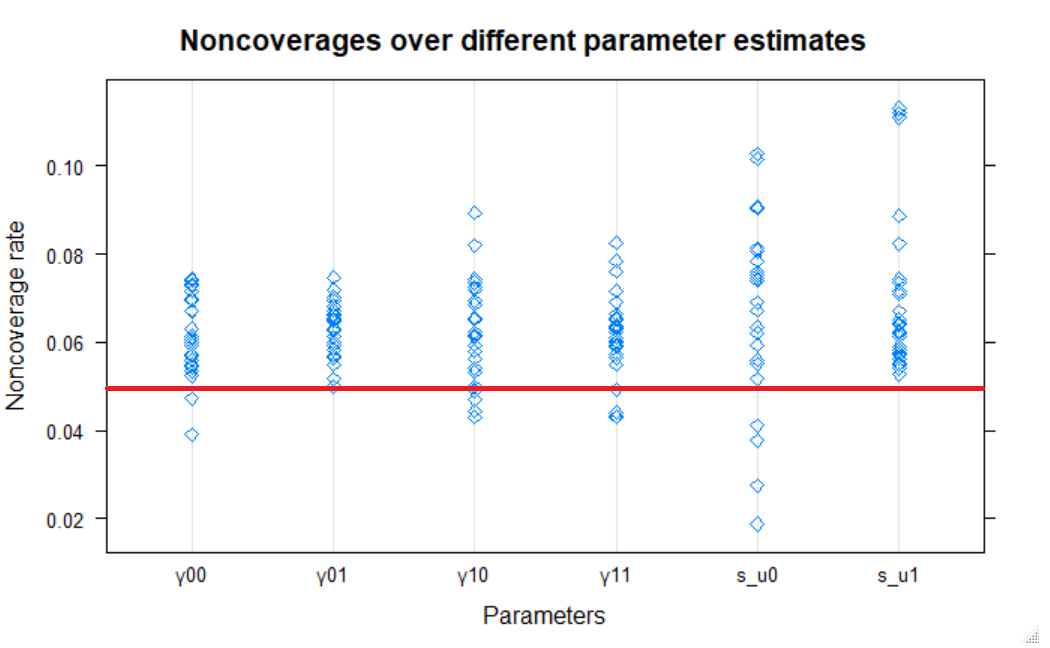
\includegraphics[width=0.8\linewidth]{figure/noncov} \caption{Dot plots of non-coverage rates of the profile likelihood confidence interval over different parameter estimates.}\label{fig:noncov}
\end{figure}
\hypertarget{conclusion}{%
\chapter{Conclusion}\label{conclusion}}

In this study, we perform Monte Carlo simulation studies to investigate the sample behavior of estimates in a binary response multilevel model using the Laplace approximation estimation procedure. Particularly, we analyze the influence of different factors (different number of groups, different group sizes, different intra-class correlation coefficients) on the accuracy of parameter estimates (fixed effects and variance components) and their profile likelihood confidence intervals.

Despite the limitations of simulation studies, our findings can offer some suggestions for sample size selection in multilevel logistic regression. With a group of 50 and group size 30, we found that the non-coverage rates for fixed effect parameters range from \(4.7\%\) to \(7.3\%\) and for level-2 variance components from \(5.7\%\) to \(7.8\%\). This is clearly different from the nominal \(5\%\), however, in practice probably acceptable (Maas \& Hox, 2005). Besides, with this sample size, the model convergence rate is almost \(100\%\), and the bias of variance components are less \(6\%\). Thus, based on our findings, we recommend a minimum of 50 groups with at least 30 units per group.

In our study, we assumed group level residuals are normally distributed. This may not be the case always. Our results are comparable with the simulation results reported by Maas \& Hox (2005), Moineddin et al. (2007), and Paccagnella (2011), when only those conditions are considered that are similar to the conditions in our simulations.
The results of some simulation studies, reviewed in this project, may appear somewhat inconsistent. However, this is probably the result of using different simulation designs and different simulated conditions.

The main findings from this research can be summarized as follows:
\begin{itemize}
\item
  The estimates of the regression coefficients are always unbiased, even with small sample sizes, except some cases on level-2 variable coefficients.
\item
  The variance components are always underestimated, even with 100 groups and 50 individuals. However, the bias decreases with the increase in number of groups, and with number of groups 50 and group size 50 this bias is less than \(5\%\).
\item
  The mean non-coverage rate for profile likelihood confidence interval is \(6.39\%\), and non-coverage rates are more close to \(6\%\), than the nominal value \(5\%\).
\item
  In some cases, profile likelihood confidence interval performs poorly for the variance components (e.g., the three cases for 100 groups with 5 individuals per group). This suggests, there might be other factors that influence the coverage rate of profile likelihood confidence interval.
\end{itemize}
\appendix

\hypertarget{r-codes-used-in-this-study}{%
\chapter{R codes used in this study}\label{r-codes-used-in-this-study}}

\small
\begin{verbatim}
library(lme4)

# Setting the parameters values
g_00 <- -1
g_01 <- 0.3
g_10 <- 0.3
g_11 <- 0.3

s2_1 <- 1                   # Variance standardized to 1
s01  <- 0                   # Covariance assumed zero
s2_e <- (pi^2)/3            # Variance of the logistic distribution

# Function for simulating data from two-level logistic regression model

sim_fun <- function(J, n_j, ICC){
  s2_0 <- s2_e / (1/ICC-1)  # Variance corresponding to specific ICC
  
  n_j <- rep(n_j, J)  # Number of individuals in jth group
  N <- sum(n_j)       # Number of groups
  
  # Simulate the covariate values for this sample size.
  
  z <- rnorm(J)
  x <- rnorm(N)
  
  # Generate (u_0j, u_1j) from a bivariate normal 
  
  mu <- c(0, 0)
  sig <- matrix(c(s2_0, s01, s01, s2_1), ncol = 2)
  u <- MASS::mvrnorm(J, mu = mu, Sigma = sig)
  
  # Now form the linear predictor.  First, the group-level predictor. 
  # There are J of these.
  
  pi_0 <- g_00 + g_01*z + as.vector(u[,1])
  pi_1 <- g_10 + g_11*z + as.vector(u[,2])
  eta <- rep(pi_0, n_j) + rep(pi_1, n_j) * x
  
  # Transform back to the probability scale.
  
  p <- exp(eta) / (1+exp(eta))
  
  # Simulate a Bernoulli from each individual distribution.
  
  y <- rbinom(N, 1, p)
  
  sim_data <- data.frame(Y=y, X=x, Z=rep(z,n_j), group=rep(1:J,n_j))
}
# End of the function 'sim_fun'

# Function for calculating percentage relative bias of the parameter estimates
# and calculating non-coverage rates.

analysis <- function(J, n_j, ICC) {
  sim_dat <- sim_fun(J, n_j, ICC)
  fit <- glmer(Y ~ X + Z + X:Z + (X||group), family=binomial, data=sim_dat,
               control=glmerControl(optCtrl=list(maxfun=2e5)))
  
  s2_0 <- s2_e / (1/ICC-1)  ##variance corresponding to specific ICC
  
  true_val <- c(g_00, g_10, g_01, g_11, sqrt(s2_0), 1)
  theta_hat <- c(as.numeric(fixef(fit)), as.data.frame(VarCorr(fit))[,5])
  perc_rel_bias <- ((theta_hat-true_val)/true_val)*100
  
  ci_profile <- confint.merMod(object = fit, method = "profile", quiet = TRUE)
  
  nc_u0  <- ifelse (ci_profile[1] < sqrt(s2_0) & ci_profile[7]  > sqrt(s2_0), 0, 1)
  nc_u1  <- ifelse (ci_profile[2] < sqrt(s2_1) & ci_profile[8]  > sqrt(s2_1), 0, 1)
  nc_int <- ifelse (ci_profile[3] < g_00       & ci_profile[9]  > g_00,       0, 1)
  nc_x   <- ifelse (ci_profile[4] < g_10       & ci_profile[10] > g_10,       0, 1)
  nc_z   <- ifelse (ci_profile[5] < g_01       & ci_profile[11] > g_01,       0, 1)
  nc_xz  <- ifelse (ci_profile[6] < g_11       & ci_profile[12] > g_11,       0, 1)
  
  noncoverage <- c(nc_int, nc_x, nc_z, nc_xz, nc_u0, nc_u1)
  return (c(perc_rel_bias, noncoverage))
}
# End of the function 'analysis'

# Combination 01:
c01 <- replicate(1000, tryCatch(analysis(30, 5, 0.1), error=function(err) rep(NA,12)))
r <- rowMeans(apply(c01, 2, unlist), na.rm = TRUE)
perc_conv <- 1 - sum(is.na(c01[1,]))/1000

# Combination 02:
c02 <- replicate(1000, tryCatch(analysis(30, 5, 0.2), error=function(err) rep(NA,12)))
r <- rbind(r, rowMeans(apply(c02, 2, unlist), na.rm = TRUE))
perc_conv <- c(perc_conv, 1 - sum(is.na(c02[1,]))/1000)

# Combination 03:
c03 <- replicate(1000, tryCatch(analysis(30, 5, 0.3), error=function(err) rep(NA,12)))
r <- rbind(r, rowMeans(apply(c03, 2, unlist), na.rm = TRUE))
perc_conv <- c(perc_conv, 1 - sum(is.na(c03[1,]))/1000)

# Combination 04:
c04 <- replicate(1000, tryCatch(analysis(30, 30, 0.1), error=function(err) rep(NA,12)))
r <- rbind(r, rowMeans(apply(c04, 2, unlist), na.rm = TRUE))
perc_conv <- c(perc_conv, 1 - sum(is.na(c04[1,]))/1000)

# Combination 05:
c05 <- replicate(1000, tryCatch(analysis(30, 30, 0.2), error=function(err) rep(NA,12)))
r <- rbind(r, rowMeans(apply(c05, 2, unlist), na.rm = TRUE))
perc_conv <- c(perc_conv, 1 - sum(is.na(c05[1,]))/1000)

# Combination 06:
c06 <- replicate(1000, tryCatch(analysis(30, 30, 0.3), error=function(err) rep(NA,12)))
r <- rbind(r, rowMeans(apply(c06, 2, unlist), na.rm = TRUE))
perc_conv <- c(perc_conv, 1 - sum(is.na(c06[1,]))/1000)

# Combination 07:
c07 <- replicate(1000, tryCatch(analysis(30, 50, 0.1), error=function(err) rep(NA,12)))
r <- rbind(r, rowMeans(apply(c07, 2, unlist), na.rm = TRUE))
perc_conv <- c(perc_conv, 1 - sum(is.na(c07[1,]))/1000)

# Combination 08:
c08 <- replicate(1000, tryCatch(analysis(30, 50, 0.2), error=function(err) rep(NA,12)))
r <- rbind(r, rowMeans(apply(c08, 2, unlist), na.rm = TRUE))
perc_conv <- c(perc_conv, 1 - sum(is.na(c08[1,]))/1000)

# Combination 09:
c09 <- replicate(1000, tryCatch(analysis(30, 50, 0.3), error=function(err) rep(NA,12)))
r <- rbind(r, rowMeans(apply(c09, 2, unlist), na.rm = TRUE))
perc_conv <- c(perc_conv, 1 - sum(is.na(c09[1,]))/1000)

# Combination 10:
c10 <- replicate(1000, tryCatch(analysis(50, 5, 0.1), error=function(err) rep(NA,12)))
r <- rbind(r, rowMeans(apply(c10, 2, unlist), na.rm = TRUE))
perc_conv <- c(perc_conv, 1 - sum(is.na(c10[1,]))/1000)

# Combination 11:
c11 <- replicate(1000, tryCatch(analysis(50, 5, 0.2), error=function(err) rep(NA,12)))
r <- rbind(r, rowMeans(apply(c11, 2, unlist), na.rm = TRUE))
perc_conv <- c(perc_conv, 1 - sum(is.na(c11[1,]))/1000)

# Combination 12:
c12 <- replicate(1000, tryCatch(analysis(50, 5, 0.3), error=function(err) rep(NA,12)))
r <- rbind(r, rowMeans(apply(c12, 2, unlist), na.rm = TRUE))
perc_conv <- c(perc_conv, 1 - sum(is.na(c12[1,]))/1000)

# Combination 13:
c13 <- replicate(1000, tryCatch(analysis(50, 30, 0.1), error=function(err) rep(NA,12)))
r <- rbind(r, rowMeans(apply(c13, 2, unlist), na.rm = TRUE))
perc_conv <- c(perc_conv, 1 - sum(is.na(c13[1,]))/1000)

# Combination 14:
c14 <- replicate(1000, tryCatch(analysis(50, 30, 0.2), error=function(err) rep(NA,12)))
r <- rbind(r, rowMeans(apply(c14, 2, unlist), na.rm = TRUE))
perc_conv <- c(perc_conv, 1 - sum(is.na(c14[1,]))/1000)

# Combination 15:
c15 <- replicate(1000, tryCatch(analysis(50, 30, 0.3), error=function(err) rep(NA,12)))
r <- rbind(r, rowMeans(apply(c15, 2, unlist), na.rm = TRUE))
perc_conv <- c(perc_conv, 1 - sum(is.na(c15[1,]))/1000)

# Combination 16:
c16 <- replicate(1000, tryCatch(analysis(50, 50, 0.1), error=function(err) rep(NA,12)))
r <- rbind(r, rowMeans(apply(c16, 2, unlist), na.rm = TRUE))
perc_conv <- c(perc_conv, 1 - sum(is.na(c16[1,]))/1000)

# Combination 17:
c17 <- replicate(1000, tryCatch(analysis(50, 50, 0.2), error=function(err) rep(NA,12)))
r <- rbind(r, rowMeans(apply(c17, 2, unlist), na.rm = TRUE))
perc_conv <- c(perc_conv, 1 - sum(is.na(c17[1,]))/1000)

# Combination 18:
c18 <- replicate(1000, tryCatch(analysis(50, 50, 0.3), error=function(err) rep(NA,12)))
r <- rbind(r, rowMeans(apply(c18, 2, unlist), na.rm = TRUE))
perc_conv <- c(perc_conv, 1 - sum(is.na(c18[1,]))/1000)

# Combination 19:
c19 <- replicate(1000, tryCatch(analysis(100, 5, 0.1), error=function(err) rep(NA,12)))
r <- rbind(r, rowMeans(apply(c19, 2, unlist), na.rm = TRUE))
perc_conv <- c(perc_conv, 1 - sum(is.na(c19[1,]))/1000)

# Combination 20:
c20 <- replicate(1000, tryCatch(analysis(100, 5, 0.2), error=function(err) rep(NA,12)))
r <- rbind(r, rowMeans(apply(c20, 2, unlist), na.rm = TRUE))
perc_conv <- c(perc_conv, 1 - sum(is.na(c20[1,]))/1000)

# Combination 21:
c21 <- replicate(1000, tryCatch(analysis(100, 5, 0.3), error=function(err) rep(NA,12)))
r <- rbind(r, rowMeans(apply(c21, 2, unlist), na.rm = TRUE))
perc_conv <- c(perc_conv, 1 - sum(is.na(c21[1,]))/1000)

# Combination 22:
c22 <- replicate(1000, tryCatch(analysis(100, 30, 0.1), error=function(err) rep(NA,12)))
r <- rbind(r, rowMeans(apply(c22, 2, unlist), na.rm = TRUE))
perc_conv <- c(perc_conv, 1 - sum(is.na(c22[1,]))/1000)

# Combination 23:
c23 <- replicate(1000, tryCatch(analysis(100, 30, 0.2), error=function(err) rep(NA,12)))
r <- rbind(r, rowMeans(apply(c23, 2, unlist), na.rm = TRUE))
perc_conv <- c(perc_conv, 1 - sum(is.na(c23[1,]))/1000)

# Combination 24:
c24 <- replicate(1000, tryCatch(analysis(100, 30, 0.3), error=function(err) rep(NA,12)))
r <- rbind(r, rowMeans(apply(c24, 2, unlist), na.rm = TRUE))
perc_conv <- c(perc_conv, 1 - sum(is.na(c24[1,]))/1000)

# Combination 25:
c25 <- replicate(1000, tryCatch(analysis(100, 50, 0.1), error=function(err) rep(NA,12)))
r <- rbind(r, rowMeans(apply(c25, 2, unlist), na.rm = TRUE))
perc_conv <- c(perc_conv, 1 - sum(is.na(c25[1,]))/1000)

# Combination 26:
c26 <- replicate(1000, tryCatch(analysis(100, 50, 0.2), error=function(err) rep(NA,12)))
r <- rbind(r, rowMeans(apply(c26, 2, unlist), na.rm = TRUE))
perc_conv <- c(perc_conv, 1 - sum(is.na(c26[1,]))/1000)

# Combination 27:
c27 <- replicate(1000, tryCatch(analysis(100, 50, 0.3), error=function(err) rep(NA,12)))
r <- rbind(r, rowMeans(apply(c27, 2, unlist), na.rm = TRUE))
perc_conv <- c(perc_conv, 1 - sum(is.na(c27[1,]))/1000)

r[,1:6]        # Relative bias of the six estimates
r[,7:12]       # Non-coverage rates of profile CI of the six estimates
perc_conv*100  # Percentages of Convergence in the 27 conditions

\end{verbatim}
\backmatter

\hypertarget{references}{%
\chapter*{References}\label{references}}
\addcontentsline{toc}{chapter}{References}

\markboth{References}{References}

\noindent

\setlength{\parindent}{-0.20in}
\setlength{\leftskip}{0.20in}
\setlength{\parskip}{8pt}

\hypertarget{refs}{}
\leavevmode\hypertarget{ref-akter2018effect}{}%
Akter, N. J., \& Khan, M. H. R. (2018). Effect of sample size on the profile likelihood estimates for two-stage hierarchical linear models. \emph{Journal of Biomedical Analytics}, \emph{1}(2), 81--89.

\leavevmode\hypertarget{ref-austin2005bias}{}%
Austin, P. C. (2005). Bias in penalized quasi-likelihood estimation in random effects logistic regression models when the random effects are not normally distributed. \emph{Communications in Statistics-Simulation and Computation}, \emph{34}(3), 549--565.

\leavevmode\hypertarget{ref-bates2010lme4}{}%
Bates, D. M. (2010). Lme4: Mixed-effects modeling with r.

\leavevmode\hypertarget{ref-breslow1993approximate}{}%
Breslow, N. E., \& Clayton, D. G. (1993). Approximate inference in generalized linear mixed models. \emph{Journal of the American Statistical Association}, \emph{88}(421), 9--25.

\leavevmode\hypertarget{ref-breslow1995bias}{}%
Breslow, N. E., \& Lin, X. (1995). Bias correction in generalised linear mixed models with a single component of dispersion. \emph{Biometrika}, \emph{82}(1), 81--91.

\leavevmode\hypertarget{ref-clarke2007addressing}{}%
Clarke, P., \& Wheaton, B. (2007). Addressing data sparseness in contextual population research: Using cluster analysis to create synthetic neighborhoods. \emph{Sociological Methods \& Research}, \emph{35}(3), 311--351.

\leavevmode\hypertarget{ref-garrett2011}{}%
Fitzmaurice, G. M., Laird, N. M., \& Ware, J. H. (2011). \emph{Applied longitudinal analysis} (2nd ed.). Wiley.

\leavevmode\hypertarget{ref-goldstein2003}{}%
Goldstein, H. (2003). \emph{Multilevel statistical models} (3rd ed.). London, UK: Arnold Publishers.

\leavevmode\hypertarget{ref-goldstein1996improved}{}%
Goldstein, H., \& Rasbash, J. (1996). Improved approximations for multilevel models with binary responses. \emph{Journal of the Royal Statistical Society: Series A (Statistics in Society)}, \emph{159}(3), 505--513.

\leavevmode\hypertarget{ref-gulliford1999components}{}%
Gulliford, M. C., Ukoumunne, O. C., \& Chinn, S. (1999). Components of variance and intraclass correlations for the design of community-based surveys and intervention studies: Data from the health survey for england 1994. \emph{American Journal of Epidemiology}, \emph{149}(9), 876--883.

\leavevmode\hypertarget{ref-guo2000multilevel}{}%
Guo, G., \& Zhao, H. (2000). Multilevel modeling for binary data. \emph{Annual Review of Sociology}, \emph{26}(1), 441--462.

\leavevmode\hypertarget{ref-handayani2017comparative}{}%
Handayani, D., Notodiputro, K. A., Sadik, K., \& Kurnia, A. (2017). A comparative study of approximation methods for maximum likelihood estimation in generalized linear mixed models (glmm). In \emph{AIP conference proceedings} (Vol. 1827, p. 020033). AIP Publishing.

\leavevmode\hypertarget{ref-hox1998multilevel}{}%
Hox, J. (1998). Multilevel modeling: When and why. In \emph{Classification, data analysis, and data highways} (pp. 147--154). Springer.

\leavevmode\hypertarget{ref-joophox2010}{}%
Hox, J. J. (2010). \emph{Multilevel analysis: Techniques and applications, second edition (quantitative methodology series)}. Routledge. Retrieved from \url{https://www.xarg.org/ref/a/1848728468/}

\leavevmode\hypertarget{ref-kreft1996}{}%
Kreft, I. G. G. (1996). Are multilevel techniques necessary? An overview, including simulation studies. Unpublished manuscript, California State University at Los Angeles. Retrieved July 6, 2005 from http://www.calstatela.edu/faculty/ikreft/quarterly.html.

\leavevmode\hypertarget{ref-lesaffre2001effect}{}%
Lesaffre, E., \& Spiessens, B. (2001). On the effect of the number of quadrature points in a logistic random effects model: An example. \emph{Journal of the Royal Statistical Society: Series C (Applied Statistics)}, \emph{50}(3), 325--335.

\leavevmode\hypertarget{ref-maas2004robustness}{}%
Maas, C. J., \& Hox, J. J. (2004). Robustness issues in multilevel regression analysis. \emph{Statistica Neerlandica}, \emph{58}(2), 127--137.

\leavevmode\hypertarget{ref-maas2005sufficient}{}%
Maas, C. J., \& Hox, J. J. (2005). Sufficient sample sizes for multilevel modeling. \emph{Methodology}, \emph{1}(3), 86--92.

\leavevmode\hypertarget{ref-mcneish2016estimation}{}%
McNeish, D. (2016). Estimation methods for mixed logistic models with few clusters. \emph{Multivariate Behavioral Research}, \emph{51}(6), 790--804.

\leavevmode\hypertarget{ref-moineddin2007simulation}{}%
Moineddin, R., Matheson, F. I., \& Glazier, R. H. (2007). A simulation study of sample size for multilevel logistic regression models. \emph{BMC Medical Research Methodology}, \emph{7}(1), 34.

\leavevmode\hypertarget{ref-mok95}{}%
Mok, M. (1995). \emph{Sample size requirements for 2-level designs in educational research}.

\leavevmode\hypertarget{ref-paccagnella2011sample}{}%
Paccagnella, O. (2011). Sample size and accuracy of estimates in multilevel models. \emph{Methodology}.

\leavevmode\hypertarget{ref-raud2002}{}%
Raudenbush, S. W., \& Bryk, A. S. (2002). \emph{Hierarchical linear models: Applications and data analysis methods} (2nd ed.). Thousand Oaks, CA: Sage Publications.

\leavevmode\hypertarget{ref-raudenbush2000maximum}{}%
Raudenbush, S. W., Yang, M.-L., \& Yosef, M. (2000). Maximum likelihood for generalized linear models with nested random effects via high-order, multivariate laplace approximation. \emph{Journal of Computational and Graphical Statistics}, \emph{9}(1), 141--157.

\leavevmode\hypertarget{ref-sastry2006design}{}%
Sastry, N., Ghosh-Dastidar, B., Adams, J., \& Pebley, A. R. (2006). The design of a multilevel survey of children, families, and communities: The los angeles family and neighborhood survey. \emph{Social Science Research}, \emph{35}(4), 1000--1024.

\leavevmode\hypertarget{ref-snijders1999multilevel}{}%
Snijders, T., \& Bosker, R. (1999). \emph{Multilevel analysis: An introduction to basic and advanced multilevel modeling.} SAGE Publications.

\leavevmode\hypertarget{ref-sommet2017keep}{}%
Sommet, N., \& Morselli, D. (2017). Keep calm and learn multilevel logistic modeling: A simplified three-step procedure using stata, r, mplus, and spss. \emph{International Review of Social Psychology}, \emph{30}(1).

\leavevmode\hypertarget{ref-venzon1988}{}%
Venzon, D. J., \& Moolgavkar, S. H. (1988). A method for computing profile-likelihood-based confidence intervals. \emph{Applied Statistics}, \emph{37}(1), 87. \url{http://doi.org/10.2307/2347496}


% Index?

\end{document}
